\documentclass[11pt]{article}
\usepackage[utf8]{inputenc}
\usepackage[spanish]{babel}
\decimalpoint
\usepackage{amsmath}
\usepackage{amsthm}
\usepackage{amssymb}
\usepackage{graphicx}
\usepackage[margin=0.8in]{geometry}
\usepackage{fancyhdr}
\usepackage[inline]{enumitem}
\usepackage{float}
\usepackage{cancel}
\usepackage{bigints}
\usepackage{listings}
\usepackage{xcolor}
\usepackage{listingsutf8}
\usepackage{algpseudocode}
\usepackage{algorithm}
\usepackage{apacite}
\usepackage{tcolorbox}
\usepackage{multicol}
\usepackage{tipa}
\usepackage{caption} 
\pagestyle{fancy}
\usepackage{hyperref}
\usepackage{mathtools}% http://ctan.org/pkg/mathtools
\hypersetup{
    colorlinks,
    citecolor=black,
    filecolor=black,
    linkcolor=black,
    urlcolor=black
}
\newcommand{\xvdash}[1]{%
	\vdash^{\mkern-10mu\scriptscriptstyle\rule[-.9ex]{0pt}{0pt}#1}%
}
\setlength{\headheight}{15pt} 
\lhead{Atractores y Expresiones Regulares para la regla 22 y 54}
\rhead{\thepage}
\lfoot{ESCOM-IPN}
\renewcommand{\footrulewidth}{0.5pt}
\setlength{\parskip}{0.5em}
\newcommand{\ve}[1]{\overrightarrow{#1}}
\newcommand{\abs}[1]{\left\lvert #1 \right\lvert}
\newcommand{\blank}{\text{\textcrb}}
\date{\today}
\title{Reporte Final.- Atractores y Expresiones Regulares para la regla 22 y 54}
\author{Sanchez Mendez Edmundo Josue}

\lstdefinestyle{customc}{
	belowcaptionskip=1\baselineskip,
	breaklines=true,
	frame=L,
	xleftmargin=\parindent,
	language=C++,
	showstringspaces=false,
	basicstyle=\ttfamily,
	keywordstyle=\bfseries\color{green!40!black},
	commentstyle=\itshape\color{purple!40!black},
	identifierstyle=\color{blue},
	numbers=left,
	stringstyle=\color{orange},
}

\lstset{escapechar=@,style=customc,tabsize=3,language=C++}

\bibliographystyle{apacite}
\begin{document}
		\begin{titlepage}
			\begin{center}
				
				% Upper part of the page. The '~' is needed because \\
				% only works if a paragraph has started.
				
				\noindent
				\begin{minipage}{0.5\textwidth}
					\begin{flushleft} \large
						
\includegraphics[width=0.5\textwidth]{resources/ipn.png}
					\end{flushleft}
				\end{minipage}%
				\begin{minipage}{0.55\textwidth}
					\begin{flushright} \large
						
\includegraphics[width=0.5\textwidth]{resources/escom.png}
					\end{flushright}
				\end{minipage}
				
				\textsc{\LARGE Instituto Politécnico Nacional}\\[0.5cm]
				
				\textsc{\Large Escuela Superior de Cómputo}\\[1cm]
				
				% Title
				
				{ \huge Reporte Final.- Atractores y Expresiones Regulares para la regla 22 y 54  \\[1cm] }
				
				{ \Large Unidad de aprendizaje: Computing Selected Topics} \\[1cm]
				
				{ \Large Grupo: 3CM19 } \\[1cm]
				
				\noindent
				\begin{minipage}{0.5\textwidth}
					\begin{flushleft} \large
						\emph{Alumno:} \\
						Sanchez Mendez Edmundo Josue
					\end{flushleft}
				\end{minipage}%
				\begin{minipage}{0.5\textwidth}
					\begin{flushright} \large
						\emph{Profesor:} \\
						Juarez Martinez Genaro
					\end{flushright}
				\end{minipage}
				
				\vfill
				% Bottom of the page
				{\large {\today}}
			\end{center}
		\end{titlepage}
	
	\titlepage
	\tableofcontents
	\newpage
	
		\begin{abstract}
		Para este reporte abarcaremos la generación de atractores y generación de cadenas aleatorias con base en las expresiones regulares para los autómatas celulares elementales con regla 22 y 54. Nuestro objetivo es poder examinar el comportamiento de estas reglas con base en sus atractores y expresiones regulares, como en el siguiente ejemplo.
	\begin{figure}[H]
			\centering
			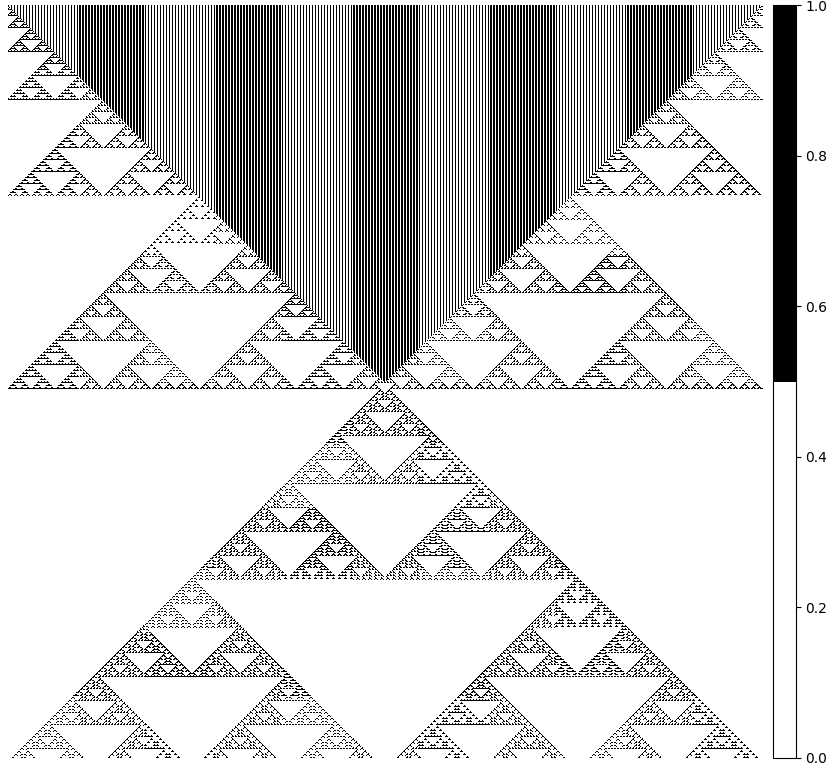
\includegraphics[scale=0.7]{resources/automata_1000x1000_r22.png}
			\caption{Autómata celular elemental de 1000 células evolucionado 1000 veces, regla 22 usando su expresión regular.}\label{fig:picture}
		\end{figure}
	\end{abstract}		
	
	\newpage
	
	\section{Introducción}
		\subsection{Atractores}
		Los atractores son un conjunto de valores numéricos hacia los cuales un sistema tiende a evolucionar, dada por una variedad de condiciones iniciales en el sistema, existen tres tipos de atractores que son los siguientes:
		 \begin{itemize}
    		 \item Atractor de punto fijo: El sistema que tenga un atractor de punto fijo tenderá a estabilizarse en un único punto.
		    \item Atractor de ciclo límite o atractor periódico: Este tipo de atractor tiende a mantenerse en un periodo o en un mismo ciclo.
		    \item Atractor caótico: Aparece en sistemas no lineales que tienen una gran sensibilidad a las condiciones. Un famoso ejemplo de estos atractores es el atractor de Lorenz.
		\end{itemize}\par
		\subsection{Expresiones regulares}		
		Las expresiones regulares nos permiten describir el lenguaje aceptado por un autómata finito, en nuestro caso buscamos ver como el uso de la expresiones regulares que describen a nuestras reglas afectan a la generación de autómatas celulares cuando se usan como condición inicial.
		\subsection{Entropia de Shannon}
		La entropía de Shannon es una de las métricas más importantes en la teoría de la información. La entropía mide la incertidumbre asociada con una variable aleatoria, es decir, el valor esperado de la información en el mensaje (en informática clásica se mide en bits).\par
El concepto fue introducido por Claude E. Shannon en el artículo ``A Mathematical Theory of Communication'' (1948). La entropía de Shannon permite estimar el número mínimo promedio de bits necesarios para codificar una cadena de símbolos en función del tamaño del alfabeto y la frecuencia de los símbolos y viene dada por la siguiente formula:
  \[ H(X) = -\sum_{i=1}^{n} P(x_i)\log_bP(x_i)\]
  En donde b es la base del logaritmo utilizado. Los valores comunes de b son 2, el número de Euler e y 10, y las unidades correspondientes de entropía son los bits para b = 2 , nats para b = e y bans para b = 10 y $P(x_i)$ como la probabilidad de un evento, para nuestro caso de estudio b=2.\par
La situación de máxima incertidumbre nos genera que sea más difícil predecir el resultado siguiente, esto es debido a que hay probabilidad uniforme. La entropía, entonces, solo puede disminuir a partir del valor asociado con la probabilidad uniforme. El caso extremo es donde un estado tiene probabilidad de 1 ya que ahí no hay incertidumbre, es decir la entropía es cero.
	\section{Expresiones Regulares}
		\subsection{Regla 22}
		La expresión regular que nos describe a la regla 22 es el siguiente:\[(0+1(01)^\ast00)(0+0(01)^\ast00)^\ast\]\par
		La expresión regular anterior nos permite poder generar cadenas aleatorias que nos servirán como condiciones iniciales para la generación de nuestros autómatas celulares elementales. Para poder visualizar como el uso de nuestra expresión regular afecta al comportamiento de nuestro autómata haremos las siguientes pruebas:
		\begin{itemize}
    		 \item Probabilidad del 50\% de unos. 
		    \item Probabilidad del 95\% de unos.
		    \item Generación de condición inicial completamente aleatoria.
		\end{itemize}\par
		Estas serán comparadas con cadenas aleatorias generadas mediante la expresión regular, todo esto se hará en un espacio de 400x400 células y se compararan tanto la imagen que nos genera el autómata así como con diferentes métricas que el programa nos proporciona.
		\subsubsection{Probabilidad del 50\% de unos}
		En la figura 2 podemos ver los valores de entrada en nuestro programa, en donde definimos un espacio de 400 x 400 células con una probabilidad de unos del 50\%		
		\begin{figure}[H]
			\centering
			\includegraphics[scale=0.5]{resources/RegEx22/50_prob_entrada.png}
			\caption{Entrada de nuestro programa para la primera prueba.}\label{fig:picture}
		\end{figure}
		En la figura 3 vemos el autómata resultante así como las métricas que el programa nos genera.
		\begin{figure}[H]
			\includegraphics[scale=0.26]{resources/RegEx22/50_prob_result.png}
			\caption{Autómata resultante con sus respectivas métricas.}\label{fig:picture}
		\end{figure}		
		En la figura 4 de igual manera que con la figura 2 podemos ver los valores de entrada de nuestro programa, en donde lo único que cambia es que en esta ocasión hacemos uso de la expresión regular de nuestra regla media la selección de la casilla con la etiqueta ``Use regular expression (rule 22 \& 54 only)''
		\begin{figure}[H]
			\centering
			\includegraphics[scale=0.5]{resources/RegEx22/50_prob_regex_entrada.png}
			\caption{Entrada de nuestro usando nuestra expresión regular r22.}\label{fig:picture}
		\end{figure}
		En la figura 5 vemos el autómata resultante así como las métricas que el programa nos genera.
		\begin{figure}[H]
			\includegraphics[scale=0.26]{resources/RegEx22/50_prob_regex_result.png}
			\caption{Autómata resultante con sus respectivas métricas.}\label{fig:picture}
		\end{figure}
		Antes de empezar con el estudio de estos dos autómatas recordar que la expresión regular se utiliza para poder generar condiciones iniciales aleatorias en las cuales tenemos un control hasta cierto punto, por lo que el autómata mostrado en la figura 5 puede variar en forma y en consecuencia en sus métricas si los comparamos con los autómatas que se generaran en las dos pruebas restantes, una vez mencionado lo anterior, comparemos los resultados.\par
		 Para nuestro autómata con probabilidad del 50\% de unos en la condición inicial vemos como 5 de nuestras 6 gráficas tienen una silueta muy similar entra ellas, vemos como el numero de unos por paso se mantienen entre los valores de 160 y 120 en donde ocasionalmente hay pasos en donde se salen de esos valores,pero nunca llegan a superar a la primera iteración en donde el numero de pasos fue de un poco mas de 200, si vemos la entropia de Shannon vemos que el valor mas alto fue de 1 y el mas bajo de 0.825 esto nos quiere decir que tenemos casi una probabilidad uniforme, esto lo podemos afirmar ya que para poder obtener el valor máximo de la entropia de shannon necesitamos probabilidades iguales, de forma general podemos decir que tenemos una gran incertidumbre y nos vemos incapaces de poder predecir el próximo estado que tomara nuestro autómata, examinando nuestra gráfica de la densidad en la columna central vemos como nos recuerda a una linea recta, es decir su crecimiento es lineal, aunque hay ciertos puntos en donde la densidad fue constante y no tenemos un patrón reconocible en nuestro autómata.\par
		 Por otro lado tenemos al autómata generado por expresión regular y a simple viste podemos observar que es un caso completamente diferente al primero ya que podemos observar cierto patrón en nuestro autómata, el cual pareciese ser la formación de un triangulo isósceles de cabeza y a sus lados patrones formados de triángulos incrustados dentro de un triangulo superior que pareciese que avanzan hasta un punto de unión formando un triangulo diferente. Observado las métricas que tenemos disponibles podemos afirmar que hay un patrón en nuestro autómata ya que las mediciones parecen repetirse por determinados ciclos, podemos ver como el numero de unos va disminuyendo a como pasan las iteraciones y por ello vemos como la densidad de la columna central llega a un máximo de 265 células con valor 1 para pasar a ser constante, vemos a la entropia iniciar con el máximo valor que puede tomar en nuestro caso de estudio a tocar el valor mas bajo, esto quiere decir que en nuestro sistema pasamos de ser incapaces de predecir el siguiente estado a poder predecir el siguiente estado de nuestro autómata.\par
		 En resumen vemos como la expresión regular en este caso nos genera un patrón muy claro en nuestro autómata y como esto influye tanto en la generación de nuestro autómata como en sus métricas en especial caso podemos ver como la entropia de nuestros dos casos de estudio son muy distintos ya que pasamos de tener una entropia casi máxima a tener una entropia casi mínima, es decir pasamos de tener una gran incertidumbre a prácticamente no tener incertidumbre.
		\subsubsection{Probabilidad del 95\% de unos}
		En la figura 6 podemos ver los valores de entrada en nuestro programa, en donde definimos un espacio de 400 x 400 células con una probabilidad de unos del 95\%		
		\begin{figure}[H]
			\centering
			\includegraphics[scale=0.5]{resources/RegEx22/95_prob_entrada.png}
			\caption{Entrada de nuestro programa para la segunda prueba.}\label{fig:picture}
		\end{figure}
		En la figura 7 vemos el autómata resultante así como las métricas que el programa nos genera.
		\begin{figure}[H]
			\includegraphics[scale=0.26]{resources/RegEx22/95_prob_result.png}
			\caption{Autómata resultante con sus respectivas métricas.}\label{fig:picture}
		\end{figure}		
		En la figura 8 de igual manera que con la figura 6 podemos ver los valores de entrada de nuestro programa, en donde lo único que cambia es que en esta ocasión hacemos uso de la expresión regular de nuestra regla media la selección de la casilla con la etiqueta ``Use regular expression (rule 22 \& 54 only)''
		\begin{figure}[H]
			\centering
			\includegraphics[scale=0.5]{resources/RegEx22/50_prob_regex_entrada.png}
			\caption{Entrada de nuestro usando nuestra expresión regular r22.}\label{fig:picture}
		\end{figure}
		En la figura 9 vemos el autómata resultante así como las métricas que el programa nos genera.
		\begin{figure}[H]
			\includegraphics[scale=0.26]{resources/RegEx22/95_prob_regex_result.png}
			\caption{Autómata resultante con sus respectivas métricas.}\label{fig:picture}
		\end{figure}
		 Para nuestro autómata con probabilidad del 95\% de unos en la condición inicial vemos como el numero de unos, el $\log_{10}$ y el valor esperado tienen una silueta muy similar entra ellas de igual forma la varianza con la entropia de Shannon, vemos como el numero de unos por paso tiene un máximo al inicio con un valor de 377 a tener un bajo en la primera iteración teniendo como valor de 9, después de este máximo y mínimo los unos tienden a crecer de una forma logarítmica ya que parece tener una asíntota horizontal en el valor 150, si vemos la entropia de Shannon podemos ver de manera clara como al inicio tenemos el valor mínimo de entropia, es decir no tenemos incertidumbre es prácticamente nula, sin embargo, con el paso de las iteraciones esta incertidumbre va aumentando hasta llegar prácticamente al punto máximo de entropia, es decir tenemos una gran incertidumbre y nos vemos incapaces de poder predecir el próximo estado que tomara nuestro autómata, examinando nuestra gráfica de la densidad en la columna central vemos como es constante el numero de 1's hasta la iteración 58 ya que desde la siguiente iteración comienza a ver un crecimiento escalonado, finalizando el análisis de este autómata podemos decir que no tenemos un patrón reconocible, sin embargo, podríamos decir que al inicio teníamos formas triangulares inscritas en un triangulo mayor pero en un punto estas figuras se perdieron.\par
		 Por otro lado tenemos al autómata generado por expresión regular y a simple viste podemos observar como comparte un patrón con el autómata de la figura 5 y es que vemos como en una parte del autómata tenemos lineas rectas que nos forman un triangulo invertido y vemos como las gráficas no se parecen en nada a la prueba de 95\% de unos. Observado las métricas que tenemos disponibles observamos una gran variación en la información que nos da el autómata y es algo completamente diferente a la prueba que estudiamos ya que en esa prueba vemos como tienden a un valor, en cambio, en este autómata podemos ver como el numero de unos va disminuyendo a como pasan las iteraciones pero no es una disminución constante si no que es como saltado y no es una reducción continua, sin embargo, vemos como la densidad de la columna central va aumentando de una forma casi lineal, pero volvemos a ver como hay puntos en donde el valor no cambia pero en su mayoría son lapsos muy pequeños, pero en la entropia podemos ver como inicia prácticamente en el máximo valor que puede tomar y después de 16 iteraciones empieza a disminuir y oscilar entre los valores 0.8 y 0.975, esto quiere decir que en nuestro sistema dentro de todas las iteraciones nos vemos incapaces de predecir el siguiente estado nuestro autómata y tenemos una alta incertidumbre.\par
		 En resumen vemos como la expresión regular en este caso no nos genera un patrón muy claro en este autómata, sin embargo, vemos como comparte un pequeño patrón con el autómata de la figura 5, asi vemos como la expresión regular sigue influyendo en la generación de nuestro autómata. En esta ocasión volvemos a ver como las métricas no coinciden, sin embargo, podemos ver como hay partes de nuestro autómata que se parecen un poco pero que nos proporcionan información distinta.\newpage
		\subsubsection{Generación de condición inicial completamente aleatoria}
		En la figura 10 podemos ver los valores de entrada en nuestro programa, en donde definimos un espacio de 400 x 400 células haciendo uso de la función random de la librería numpy de Python el cual nos generara un arreglo de determinado tamaño, en este caso de 400 células, lleno aleatoriamente de números 0 y 1.		
		\begin{figure}[H]
			\centering
			\includegraphics[scale=0.5]{resources/RegEx22/random_entrada.png}
			\caption{Entrada de nuestro programa para la tercera prueba.}\label{fig:picture}
		\end{figure}
		En la figura 11 vemos el autómata resultante así como las métricas que el programa nos genera.
		\begin{figure}[H]
			\includegraphics[scale=0.26]{resources/RegEx22/random_result.png}
			\caption{Autómata resultante con sus respectivas métricas.}\label{fig:picture}
		\end{figure}		
		En la figura 12 de igual manera que con la figura 10 podemos ver los valores de entrada de nuestro programa, en donde lo único que cambia es que en esta ocasión hacemos uso de la expresión regular de nuestra regla media la selección de la casilla con la etiqueta ``Use regular expression (rule 22 \& 54 only)''
		\begin{figure}[H]
			\centering
			\includegraphics[scale=0.5]{resources/RegEx22/50_prob_regex_entrada.png}
			\caption{Entrada de nuestro usando nuestra expresión regular r22.}\label{fig:picture}
		\end{figure}
		En la figura 13 vemos el autómata resultante así como las métricas que el programa nos genera.
		\begin{figure}[H]
			\includegraphics[scale=0.26]{resources/RegEx22/random_regex_result.png}
			\caption{Autómata resultante con sus respectivas métricas.}\label{fig:picture}
		\end{figure}
		 Para nuestro autómata generado de manera aleatoria vemos como las gráficas comparten una silueta muy similar entra, vemos como el numero de unos por paso tiene un máximo al inicio con un valor de 200 para después disminuir y rondar valores de 104 como el mas bajo a 182 como el valor mas alto, si vemos la entropia de Shannon podemos ver que volvemos a tener un patrón similar a las pruebas pasadas, en donde comenzamos con prácticamente la entropia máxima a disminuir un poco y oscilar entre los valores 0.825 y 0.9941, esto nos vuelve a indicar que tenemos incertidumbre, examinando nuestra gráfica de la densidad en la columna central vemos un crecimiento prácticamente lineal en el numero de 1's pero hay que mencionar que volvemos a ver partes en donde la gráfica de densidad es constante, finalizando el análisis de este autómata podemos decir que no tenemos un patrón reconocible a diferencia de pruebas pasadas en donde si podríamos llegar a visualizar patrones.\par
		 Por otro lado tenemos al autómata generado por expresión regular y a simple viste podemos observar como volvemos a compartir el patrón de triangulo invertido formado por lineas rectas de valores 0 y 1 intercaladas de los autómatas generados por expresión regular de las pruebas anteriores y de hecho podemos ver un gran parecido con el autómata de la figura 9 tanto en las gráficas como en el mismo autómata solo que el autómata que estamos estudiando tenemos el patrón de los triángulos incrustados en otro aún mayor pero en esta ocasión podemos ver esa patrón mas veces pero volvemos a llegar un punto en donde los  patrones desaparecen. Observado las métricas que tenemos disponibles observamos como el numero de unos tiene un máximo de 382 unos a tener un mínimo de 177 para después empezar a rondar los valores de 211 a 300 células con valor 1, sin embargo, vemos como la densidad de la columna central al inicio tienen un crecimiento lineal entre la iteración inicial hasta la 25 para después volverse constante hasta la iteración 60 en donde ya empieza a existir un incremento casi lineal pero volvemos a ver como hay partes en done es constante, pero en la entropia podemos ver que es muy similar a la vista en la figura 9 en donde vemos como inicia prácticamente en el máximo valor que puede tomar y después de 16 iteraciones empieza a disminuir y oscilar entre los valores 0.79 y 0.99, esto quiere decir que en nuestro sistema dentro de todas las iteraciones nos vemos incapaces de predecir el siguiente estado nuestro autómata y tenemos una alta incertidumbre.\par
		 Una vez visto estas tres pruebas podemos decir que la expresión regular nos genera patrones comunes entre los diferentes autómatas aun a pesar de que esta se genera de manera aleatoria, el patrón mas reconocible son las intercalaciones de columnas de ceros y unos que forman un triangulo invertido, mientras que también existe otro patrón en donde hay triángulos inscritos en un uno mayor y es común ver estos patrones juntos, también vemos como si usamos el 50\%, 95\% e inclusive la formación aleatoria nos generan autómatas en donde la mayor parte de la iteraciones tenemos una gran entropia aunque esto también lo podemos ver en la generada mediante la expresión regular aunque existen formaciones como la figura 5 en donde la entropia llega casi al mínimo valor.
		\subsection{Regla 54}
		La expresión regular que nos describe a la regla 54 es el siguiente: \[(0+1(11)^\ast10)(0+0(11)^\ast10)^\ast\]\par
		La expresión regular anterior nos permite poder generar cadenas aleatorias que nos servirán como condiciones iniciales para la generación de nuestros autómatas celulares elementales. Para poder visualizar como el uso de nuestra expresión regular afecta al comportamiento de nuestro autómata haremos las siguientes pruebas:
		\begin{itemize}
    		 \item Probabilidad del 50\% de unos. 
		    \item Probabilidad del 95\% de unos.
		    \item Generación de condición inicial completamente aleatoria.
		\end{itemize}\par
		Estas serán comparadas con cadenas aleatorias generadas mediante la expresión regular, todo esto se hará en un espacio de 400x400 células y se compararan tanto la imagen que nos genera el autómata así como con diferentes métricas que el programa nos proporciona.
 		\subsubsection{Probabilidad del 50\% de unos}
		En la figura 14 podemos ver los valores de entrada en nuestro programa, en donde definimos un espacio de 400 x 400 células con una probabilidad de unos del 50\%		
		\begin{figure}[H]
			\centering
			\includegraphics[scale=0.5]{resources/RegEx54/50_prob_entrada.png}
			\caption{Entrada de nuestro programa para la primera prueba.}\label{fig:picture}
		\end{figure}
		En la figura 15 vemos el autómata resultante así como las métricas que el programa nos genera.
		\begin{figure}[H]
			\includegraphics[scale=0.26]{resources/RegEx54/50_prob_result.png}
			\caption{Autómata resultante con sus respectivas métricas.}\label{fig:picture}
		\end{figure}		
		En la figura 16 de igual manera que con la figura 14 podemos ver los valores de entrada de nuestro programa, en donde lo único que cambia es que en esta ocasión hacemos uso de la expresión regular de nuestra regla media la selección de la casilla con la etiqueta ``Use regular expression (rule 22 \& 54 only)''
		\begin{figure}[H]
			\centering
			\includegraphics[scale=0.5]{resources/RegEx54/50_prob_regex_entrada.png}
			\caption{Entrada de nuestro usando nuestra expresión regular r54.}\label{fig:picture}
		\end{figure}
		En la figura 17 vemos el autómata resultante así como las métricas que el programa nos genera.
		\begin{figure}[H]
			\includegraphics[scale=0.26]{resources/RegEx54/50_prob_regex_result.png}
			\caption{Autómata resultante con sus respectivas métricas.}\label{fig:picture}
		\end{figure}
		Para nuestro autómata con probabilidad del 50\% de unos en la condición inicial vemos como 3 de nuestras gráficas tienen una silueta muy similar entra ellas, vemos como el numero de unos por paso se mantienen entre los valores de 123 y 258, si examinamos un poco la gráfica vemos como hay pasos intermedios en donde se encuentran prácticamente a la mitad de los valores anteriormente mencionados y si nos ponemos algo imaginativos podría llegar a parecer la gratificación de una parte de algún audio, si vemos la entropia de Shannon vemos que el valor prácticamente se mantiene en el valor mas alto que es 1 tenemos pasos intermedios en donde la entropia disminuye un poco, las partes en donde la entropia es prácticamente el valor máximo coincide con los puntos en donde el numero de 1 por paso se encuentra cercano a 200 1's por paso, esto es lógico ya que la probabilidad de los eventos sera igualmente probable provocando así la entropia mas alta, como ya sabemos al tener esta entropia tan alta tenemos una gran incertidumbre y nos vemos incapaces de poder predecir el próximo estado que tomara nuestro autómata, examinando nuestra gráfica de la densidad en la columna central vemos como nos recuerda a una linea recta, es decir su crecimiento es lineal, pero si examinamos a detalle nuestra gráfica parece una escalara en donde los escalones tienen diferente longitud, esto se debe a que hay ciertas iteaciones en donde el numero de 1's se mantiene constante, y no tenemos un patrón reconocible en nuestro autómata pero si tenemos lineas formadas por triángulos invertidos pequeños a través de todo nuestro autómata.\par
		 Por otro lado tenemos al autómata generado por expresión regular y a simple viste podemos observar que es un caso diferente al primero ya que podemos observar cierto patrón en nuestro autómata, el cual tiene triángulos invertidos compuesto de células con valor 0 al inicio, para después desaparecer, y también los triángulos que se complementan con los anteriores justo a la mitad, empiezan a generar lineas prácticamente rectas que se dirigen hacia la parte baja. Observando las métricas que tenemos disponibles podemos ver como el numero de unos tiene un comportamiento muy interesante y es que vemos como al inicio de nuestro autómata tiene un máximo de 1's teniendo un valor de 657 que disminuye a un mínimo de 42 en la iteración 2 y a partir de ahí va incrementando de una manera casi logarítmica pero con el detalle de oscilar entre los valores 184 y 525, de hecho la densidad de la columna central al inicio es constante hasta la iteración 36 ya que desde ahí empieza a tener un incremento casi lineal ya que volvemos a ver ese escalonado pero en esta ocasión es prácticamente de una iteración, vemos a la entropia iniciar con un valor de 0.41 de entropia para luego caer a 0.32 y a partir de ahí comportarse como las demás gráficas y empezar a subir prácticamente hasta el valor máximo esto quiere decir que en nuestro sistema pasamos de poder tener la capacidad de predecir el siguiente estado a ser incapaces de predecir el siguiente estado de nuestro autómata, en otras palabras pasamos de tener baja incertidumbre a tener prácticamente la máxima incertidumbre posible.\par
		 En resumen vemos como la expresión regular en este caso nos genera algo completamente a la prueba del 50\%, algo curioso de estas pruebas es que en la entropia a pesar de que el autómata generado por medio de la expresión regular tiene baja entropia al inicio pocas iteraciones después tenemos prácticamente la máxima al igual que el caso de estudio del 50\% de probabilidad, también vemos que la gráfica de la columna de densidad central ambas tienen un crecimiento casi lineal y en los autómatas nos encontramos con pequeñas columnas que atraviesan al autómata en su totalidad.\newpage
		\subsubsection{Probabilidad del 95\% de unos}
		En la figura 18 podemos ver los valores de entrada en nuestro programa, en donde definimos un espacio de 400 x 400 células con una probabilidad de unos del 95\%		
		\begin{figure}[H]
			\centering
			\includegraphics[scale=0.5]{resources/RegEx54/95_prob_entrada.png}
			\caption{Entrada de nuestro programa para la segunda prueba.}\label{fig:picture}
		\end{figure}
		En la figura 19 vemos el autómata resultante así como las métricas que el programa nos genera.
		\begin{figure}[H]
			\includegraphics[scale=0.26]{resources/RegEx54/95_prob_result.png}
			\caption{Autómata resultante con sus respectivas métricas.}\label{fig:picture}
		\end{figure}		
		En la figura 20 de igual manera que con la figura 18 podemos ver los valores de entrada de nuestro programa, en donde lo único que cambia es que en esta ocasión hacemos uso de la expresión regular de nuestra regla media la selección de la casilla con la etiqueta ``Use regular expression (rule 22 \& 54 only)''
		\begin{figure}[H]
			\centering
			\includegraphics[scale=0.5]{resources/RegEx54/50_prob_regex_entrada.png}
			\caption{Entrada de nuestro usando nuestra expresión regular r54.}\label{fig:picture}
		\end{figure}
		En la figura 21 vemos el autómata resultante así como las métricas que el programa nos genera.
		\begin{figure}[H]
			\includegraphics[scale=0.26]{resources/RegEx54/95_prob_regex_result.png}
			\caption{Autómata resultante con sus respectivas métricas.}\label{fig:picture}
		\end{figure}
		 Para nuestro autómata con probabilidad del 95\% de unos en la condición inicial vemos nos recuerda un poco al autómata de la figura 17 el cual fue generado con base en la expresión regular, ya que vemos métricas con siluetas prácticamente idénticas, de hecho a simple vista podríamos llegar a pensar en que nuestro autómata generado forma parte del autómata de la figura 17, entrando directamente en el estudio de las métricas podemos observar como el numero de unos por paso coincide con el comportamiento del autómata de la figura 17, ya que pasamos de un máximo, en este caso con valor de 386, para pasar a un mínimo de 14 unos en el paso 1, para empezar a subir en el numero de unos como si fuese una función logarítmica, solo que se mantiene oscilando entre los valores 98 como el limite inferior y de 300 como el limite superior, si vemos la entropia de Shannon podemos ver sin un duda alguna un comportamiento parecido a la entropia de nuestro autómata de la figura 17, ya que de forma general partimos de un valor muy bajo, en este caso de estudio partimos del valor 0.2189 a empezar a subir de manera muy rápida a prácticamente el valor máximo posible de entropia, de hecho entre el paso 10 al 80 tiene una oscilación en los valores pasando de la entropia máxima a una inferior, el mínimo fue de 0.70, del paso 81 en adelante vemos como decae y crece la entropia, esto entre los valores 0.80 y 0.9680, como algo interesante y al mismo tiempo curioso vemos que entre paso 81 al 400 nos recuerda un poco al electrocardiograma, por supuesto, esto en silueta, para terminar la parte de la entropia podemos decir que en nuestro sistema pasamos de poder tener la capacidad de poder saber el siguiente estado de nuestro autómata a perder dicha capacidad, en otras palabras pasamos de una incertidumbre muy baja a prácticamente la mas alta posible, por ultimo, examinando nuestra gráfica de la densidad en la columna central vemos nuevamente un comportamiento parecido con el autómata de la figura 17, en donde tenemos una parte constante de 1's para empezar a subir prácticamente de forma lineal, pero viendo de nuevo ese parte escalonada, en donde hay pasos en donde la densidad no es afectada, en este caso la parte constante es hasta el paso 11 y es ahí en donde vemos el crecimiento en la densidad de la columna central.\par
		 Por otro lado tenemos al autómata generado por expresión regular y a simple viste podemos observar una similitud con el autómata de la figura 17, tanto en comportamiento de las gráficas como en el autómata mismo, solo que en esta ocasión no tenemos una linea formada de triángulos que atraviesen todo nuestro autómata en algunos de nuestros triángulos. Observando las métricas que tenemos disponibles podemos ver como el numero de unos tiene un comportamiento muy interesante y es que vemos como al inicio de nuestro autómata tiene un máximo de 1's teniendo un valor de 667 que disminuye a un mínimo de 34 en la iteración 2 y a partir de ahí va incrementando de una manera casi logarítmica con un oscilamiento muy interesante ya que pareciese que se complementan los pasos entre si, para que a partir del paso 167 oscile entre los valores 252 y 471, de igual forma los pasos parecen complementarse, de hecho la densidad de la columna central al inicio es constante hasta la iteración 58 ya que desde ahí empieza a tener un incremento casi lineal ya que volvemos a ver ese escalonado en donde tenemos 2 pasos que comparten la misma densidad hasta el paso 230 en donde ahora 1 paso es el que comparte la densidad anterior, vemos a la entropia iniciar con un valor de 0.39 de entropia para luego caer a 0.2743 y a partir de ahí comportarse como las demás gráficas y empezar a subir prácticamente hasta el valor máximo, sin embargo, vale la pena mencionar que parece que la entropia va decayendo poco a poco, pero esto quiere decir que en nuestro sistema pasamos de poder tener la capacidad de predecir el siguiente estado a ser incapaces de predecir el siguiente estado de nuestro autómata, en otras palabras pasamos de tener baja incertidumbre a tener prácticamente la máxima incertidumbre posible.\par
		 En resumen vemos como la expresión regular en este caso nos genera algo similar a la prueba del 95\%, esto nos quiere decir que nuestra expresión regular nos genera condiciones iniciales en donde podríamos encontrar un mínimo del 95\% de unos ya que los autómatas que se generaron fueron muy similares, principalmente en el comportamiento del autómata en donde el podemos ver ciertas similitudes entre ambos, también así en el comportamiento de nuestras métricas.
		\subsubsection{Generación de condición inicial completamente aleatoria}
		En la figura 22 podemos ver los valores de entrada en nuestro programa, en donde definimos un espacio de 400 x 400 células haciendo uso de la función random de la librería numpy de Python el cual nos generara un arreglo de determinado tamaño, en este caso de 400 células, lleno aleatoriamente de números 0 y 1.		
		\begin{figure}[H]
			\centering
			\includegraphics[scale=0.5]{resources/RegEx54/random_entrada.png}
			\caption{Entrada de nuestro programa para la tercera prueba.}\label{fig:picture}
		\end{figure}
		En la figura 23 vemos el autómata resultante así como las métricas que el programa nos genera.
		\begin{figure}[H]
			\includegraphics[scale=0.26]{resources/RegEx54/random_result.png}
			\caption{Autómata resultante con sus respectivas métricas.}\label{fig:picture}
		\end{figure}		
		En la figura 12 de igual manera que con la figura 10 podemos ver los valores de entrada de nuestro programa, en donde lo único que cambia es que en esta ocasión hacemos uso de la expresión regular de nuestra regla media la selección de la casilla con la etiqueta ``Use regular expression (rule 22 \& 54 only)''
		\begin{figure}[H]
			\centering
			\includegraphics[scale=0.5]{resources/RegEx54/50_prob_regex_entrada.png}
			\caption{Entrada de nuestro usando nuestra expresión regular r22.}\label{fig:picture}
		\end{figure}
		En la figura 13 vemos el autómata resultante así como las métricas que el programa nos genera.
		\begin{figure}[H]
			\includegraphics[scale=0.26]{resources/RegEx54/random_regex_result.png}
			\caption{Autómata resultante con sus respectivas métricas.}\label{fig:picture}
		\end{figure}
		 Para nuestro autómata generado de manera aleatoria vemos como las gráficas son completamente diferentes a los autómatas generados con la misma regla anteriores, esto se debe a la generación aleatoria que tenemos y es que no tenemos control alguno, vemos como el numero de unos por paso tiene un mínimo global en el paso 3 con un valor de 149 1's por paso, y un máximo global en el paso 269 con un valor de 220 1's, si vemos la entropia de Shannon podemos ver que comenzamos con prácticamente la entropia máxima a diminuir a un mínimo global de 0.9525, que es relativamente poco, la entopia se mantiene prácticamente en el máximo por todos los pasos, esto nos vuelve a indicar que tenemos incertidumbre prácticamente máxima, examinando nuestra gráfica de la densidad en la columna central vemos un crecimiento prácticamente lineal en el numero de 1's pero hay que mencionar que volvemos a ver partes en donde la gráfica de densidad es constante, finalizando el análisis de este autómata podemos decir que no tenemos un patrón reconocible.\par
		 Por otro lado tenemos al autómata generado por expresión regular y a simple viste podemos observar como volvemos a ver un comportamiento muy similar a los autómatas generados por la expresión regular. Observado las métricas que tenemos disponibles observamos como el numero de unos tiene un máximo de 652 unos a tener un mínimo de 35 para después incrementar y empezar a rondar los valores de 152 a 500 células con valor 1, también vemos como la densidad de la columna central al inicio tienen un crecimiento constante hasta el paso 23 para después crecer de una forma linea pero volvemos a ver como hay partes en donde es constante, estudiando la entropia podemos ver que es ligeramente diferentes a las anteriormente estudiadas, aunque el inicio es similar, empezamos de valores bajos para poco después subir prácticamente al máximo, oscilar entre el valor máximo y 0.775, para después no oscilar tanto y al final, en este autómata, para que la entropia crece entre la iteración 300 y la 400 llegando a un valor de 0.965, esto quiere decir que en nuestro sistema empezamos con una baja entropia para después oscilar entre valores altos de entropia, esto nos dice que somos incapaces de predecir el siguiente estado nuestro autómata y tenemos una alta incertidumbre.\par
		 Una vez visto estas tres pruebas podemos decir que la expresión regular nos genera autómatas comunes, sin embargo, en la prueba del 95\% vemos como se nos genera un autómata muy similar a los generados por al expresión regular, al igual es similar en las métricas que se nos genera, esto nos quiere decir que nuestros autómatas que genera la expresión regular tienen una gran cantidad de 1's, volvemos a ver como el uso de la opción de generar una condición completamente aleatoria nos genera resultados completamente diferentes tanto a la expresión regular como al porcentaje de unos.	
	\section{Atractores}
	Para el desarrollo de esta parte se uso Python como lenguaje de programación, los atractores son guardados en carpetas con el nombre de regla, así también, el nombre del archivo que se genera se guarda con el siguiente formato: atractor\_'numero de la regla'\_size\_'longitud'.graphml, para poder visualizar los resultados se necesita de un programa capas de abrir archivos con formato .graphml, hay varias opciones gratis para diferentes sistemas operativos, las mas conocidas son las siguientes:
		\begin{enumerate}    
  			\item Windows
  				\begin{enumerate}
    				\item Gephi. Gratuito
    				\item yWorks yEd Graph Editor. Gratuito
    				\item Cytoscape. Gratuito
    			\end{enumerate}
  			\item MacOS
  				\begin{enumerate}
    				\item Gephi. Gratuito
    				\item yWorks yEd Graph Editor. Gratuito
    			\end{enumerate}
  			\item Linux
  				\begin{enumerate}
    				\item Gephi. Gratuito
    				\item yWorks yEd Graph Editor. Gratuito
    			\end{enumerate}
		\end{enumerate}
		Esto con el fin de proporcionar la capacidad de modificar las formas de los nodos, los vértices, colores, forma de organización entre algunas otras opciones mas. En nuestro caso se uso el programa Cytoscape el cual nos proporciona las características anteriormente mencionadas y algunas otras metras. Empecemos así con los atractores.
		\subsection{Regla 22}
		El formato sera el siguiente, primero se pondrá la imagen del atractor y después evoluciones de los nodos para ver los atractores que existen.
			\subsubsection{Tamaño 2}
			\begin{figure}[H]
			\centering
			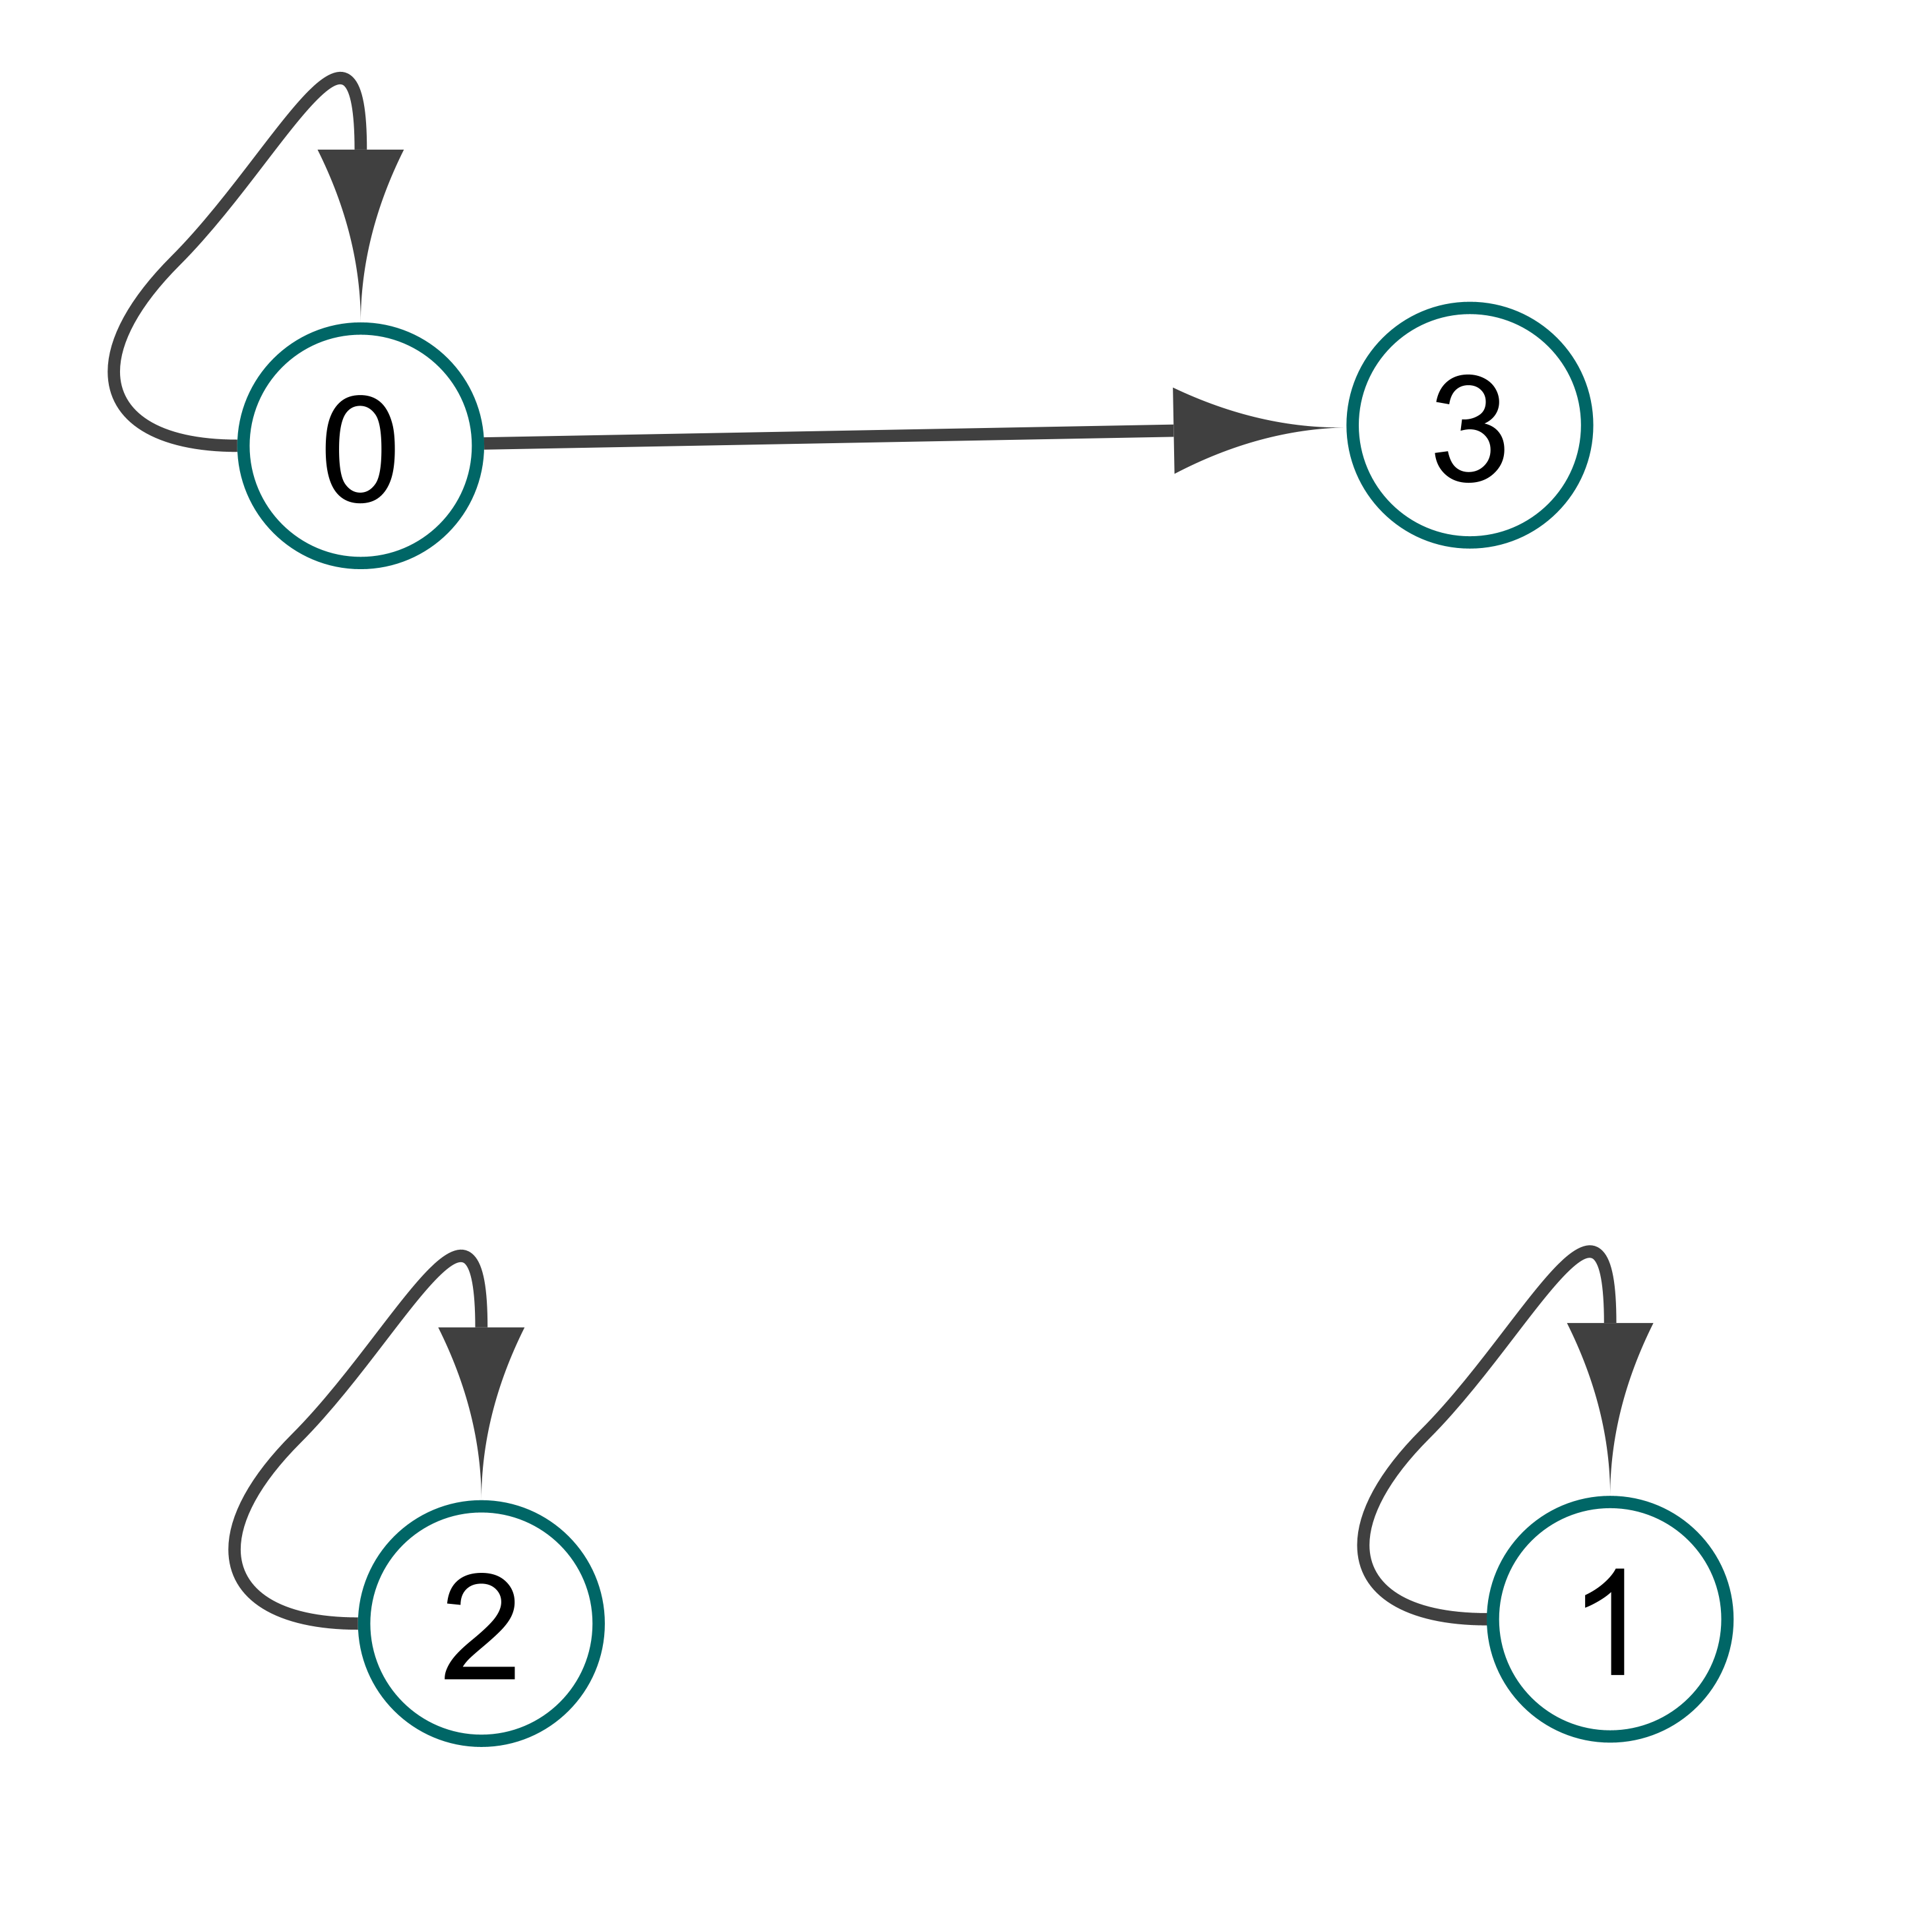
\includegraphics[scale=0.08]{resources/Atractores22/atractor_22_size_2.png}
			\caption{Atractor de tamaño 2.}\label{fig:picture}
			\end{figure}
			\begin{figure}[H]
			\centering
			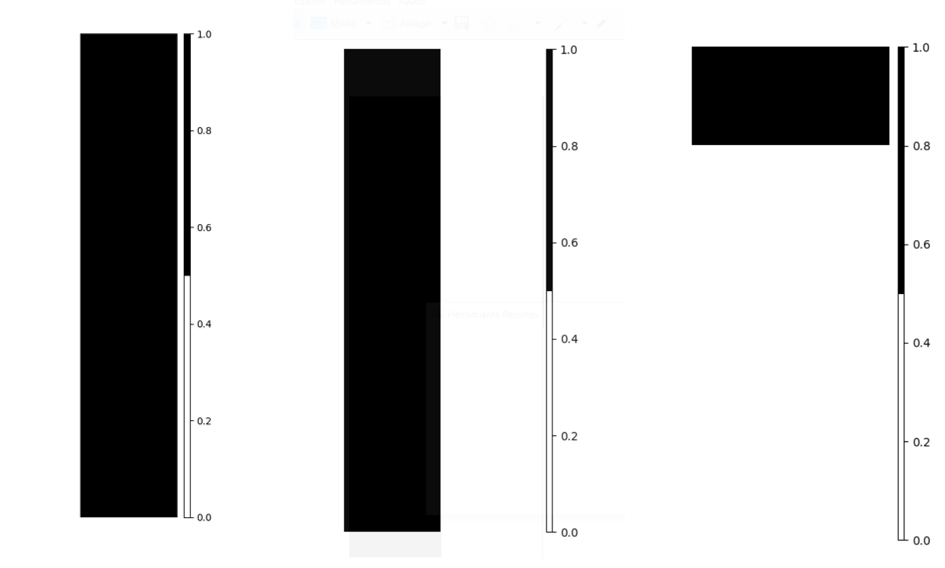
\includegraphics[scale=0.5]{resources/Atractores22/atractor_22_size_2_res.png}
			\caption{Evoluciones de los atractores.}\label{fig:picture}
			\end{figure}
			Mencionar que en la imagen 27 y durante algunos tamaños las evoluciones serán acomodadas tal que del lado izquierdo se tenga el nodo de menor numero al mayor, ya que si lo hicieramos por cada nodo simplemente no acabaríamos, mencionar que para este atractor no vemos el caso del nodo 0 ya que el nodo 3 al dirigirse al nodo 0 entra en un ciclo en donde vemos el comportamiento del nodo 0.
			\subsubsection{Tamaño 3}
			\begin{figure}[H]
			\centering
			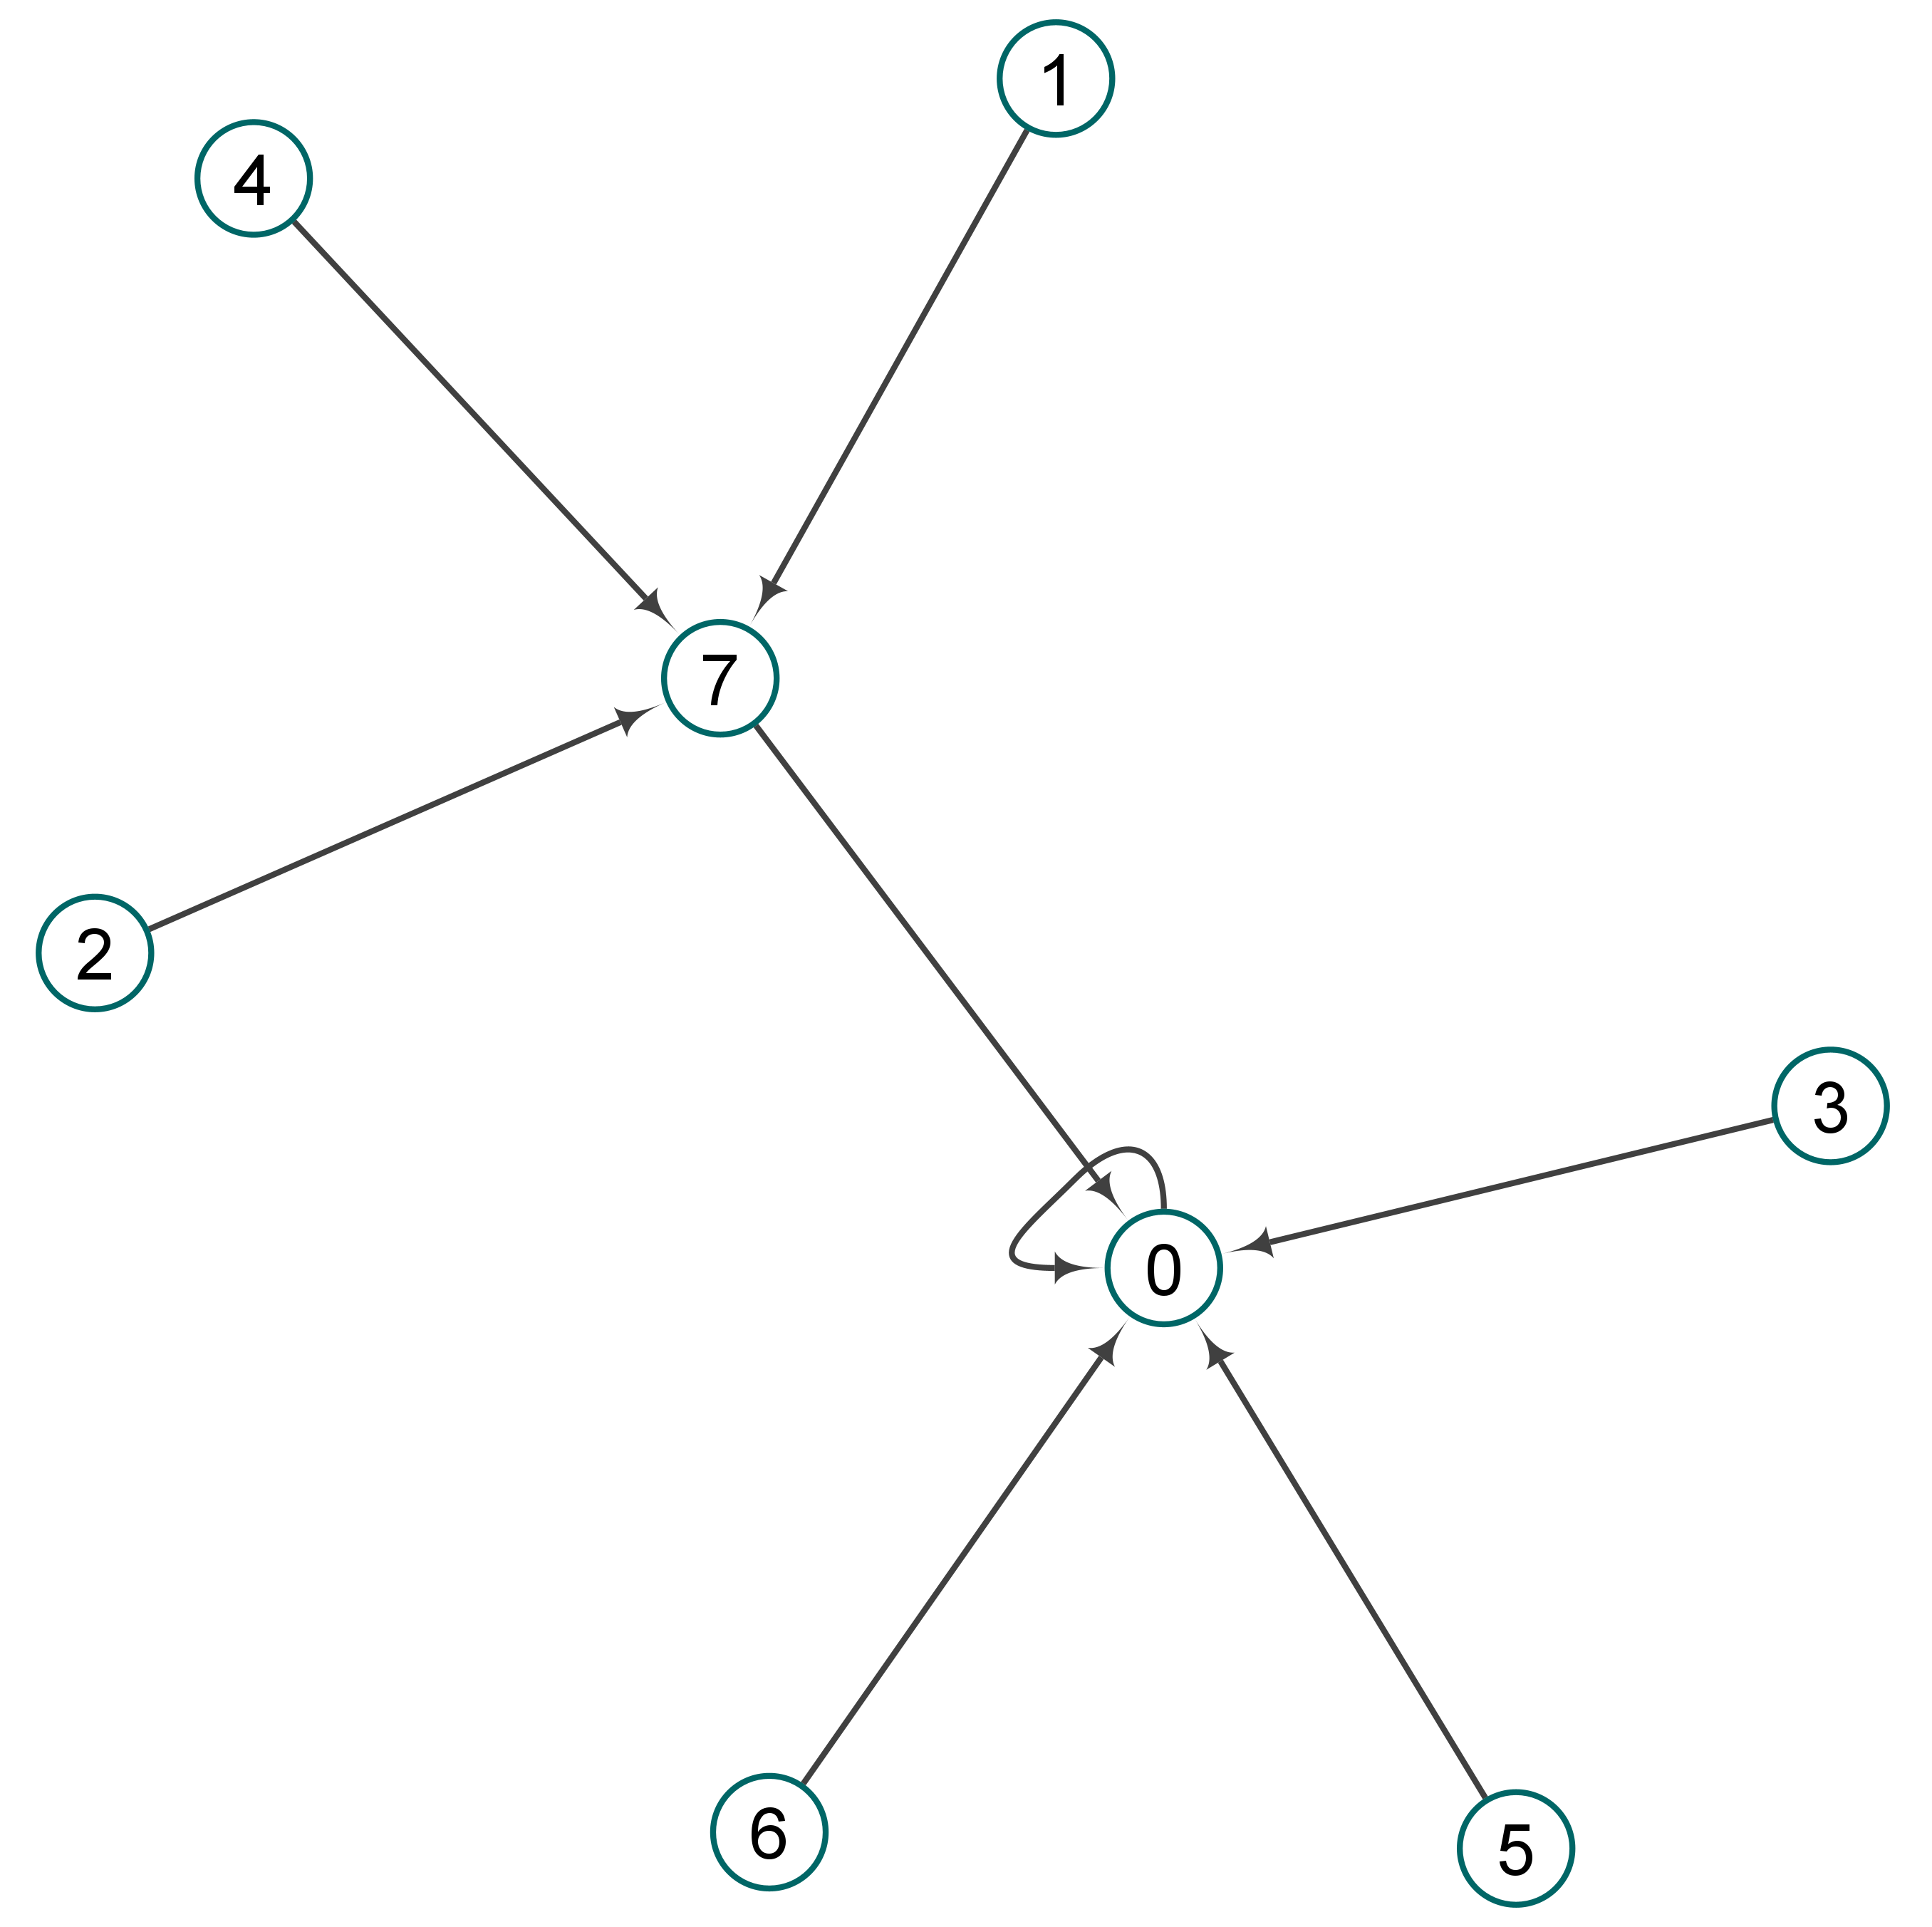
\includegraphics[scale=0.1]{resources/Atractores22/atractor_22_size_3.png}
			\caption{Atractor de tamaño 3.}\label{fig:picture}
			\end{figure}
			\begin{figure}[H]
			\centering
			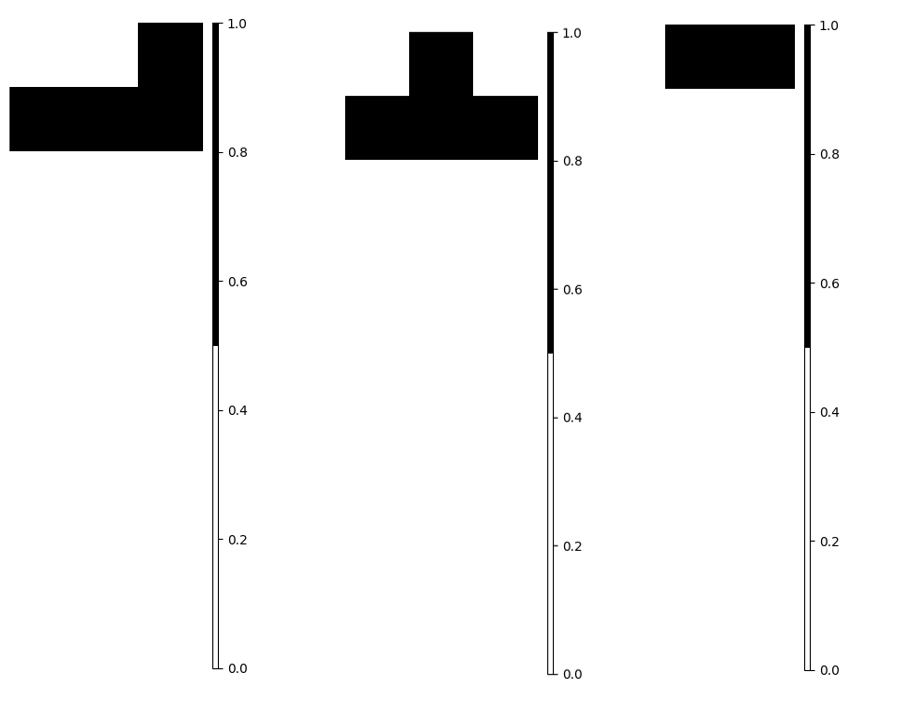
\includegraphics[scale=0.3]{resources/Atractores22/atractor_22_size_3_res.png}
			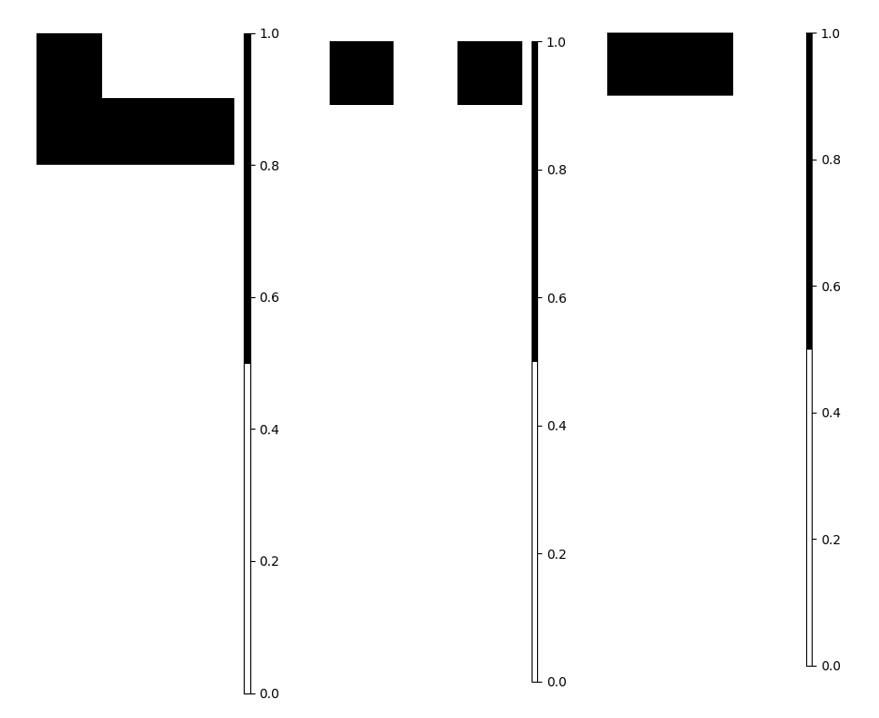
\includegraphics[scale=0.3]{resources/Atractores22/atractor_22_size_3_res1.png}
			\caption{Evoluciones de los atractores.}\label{fig:picture}
			\end{figure}
			Mencionar que para este atractor no vemos el caso del nodo 0 ya que el nodo 7, 3, 5, 6 se dirigen al nodo 0 el cual entra en un ciclo en donde vemos el comportamiento del nodo 0.
			\subsubsection{Tamaño 4}
			\begin{figure}[H]
			\centering
			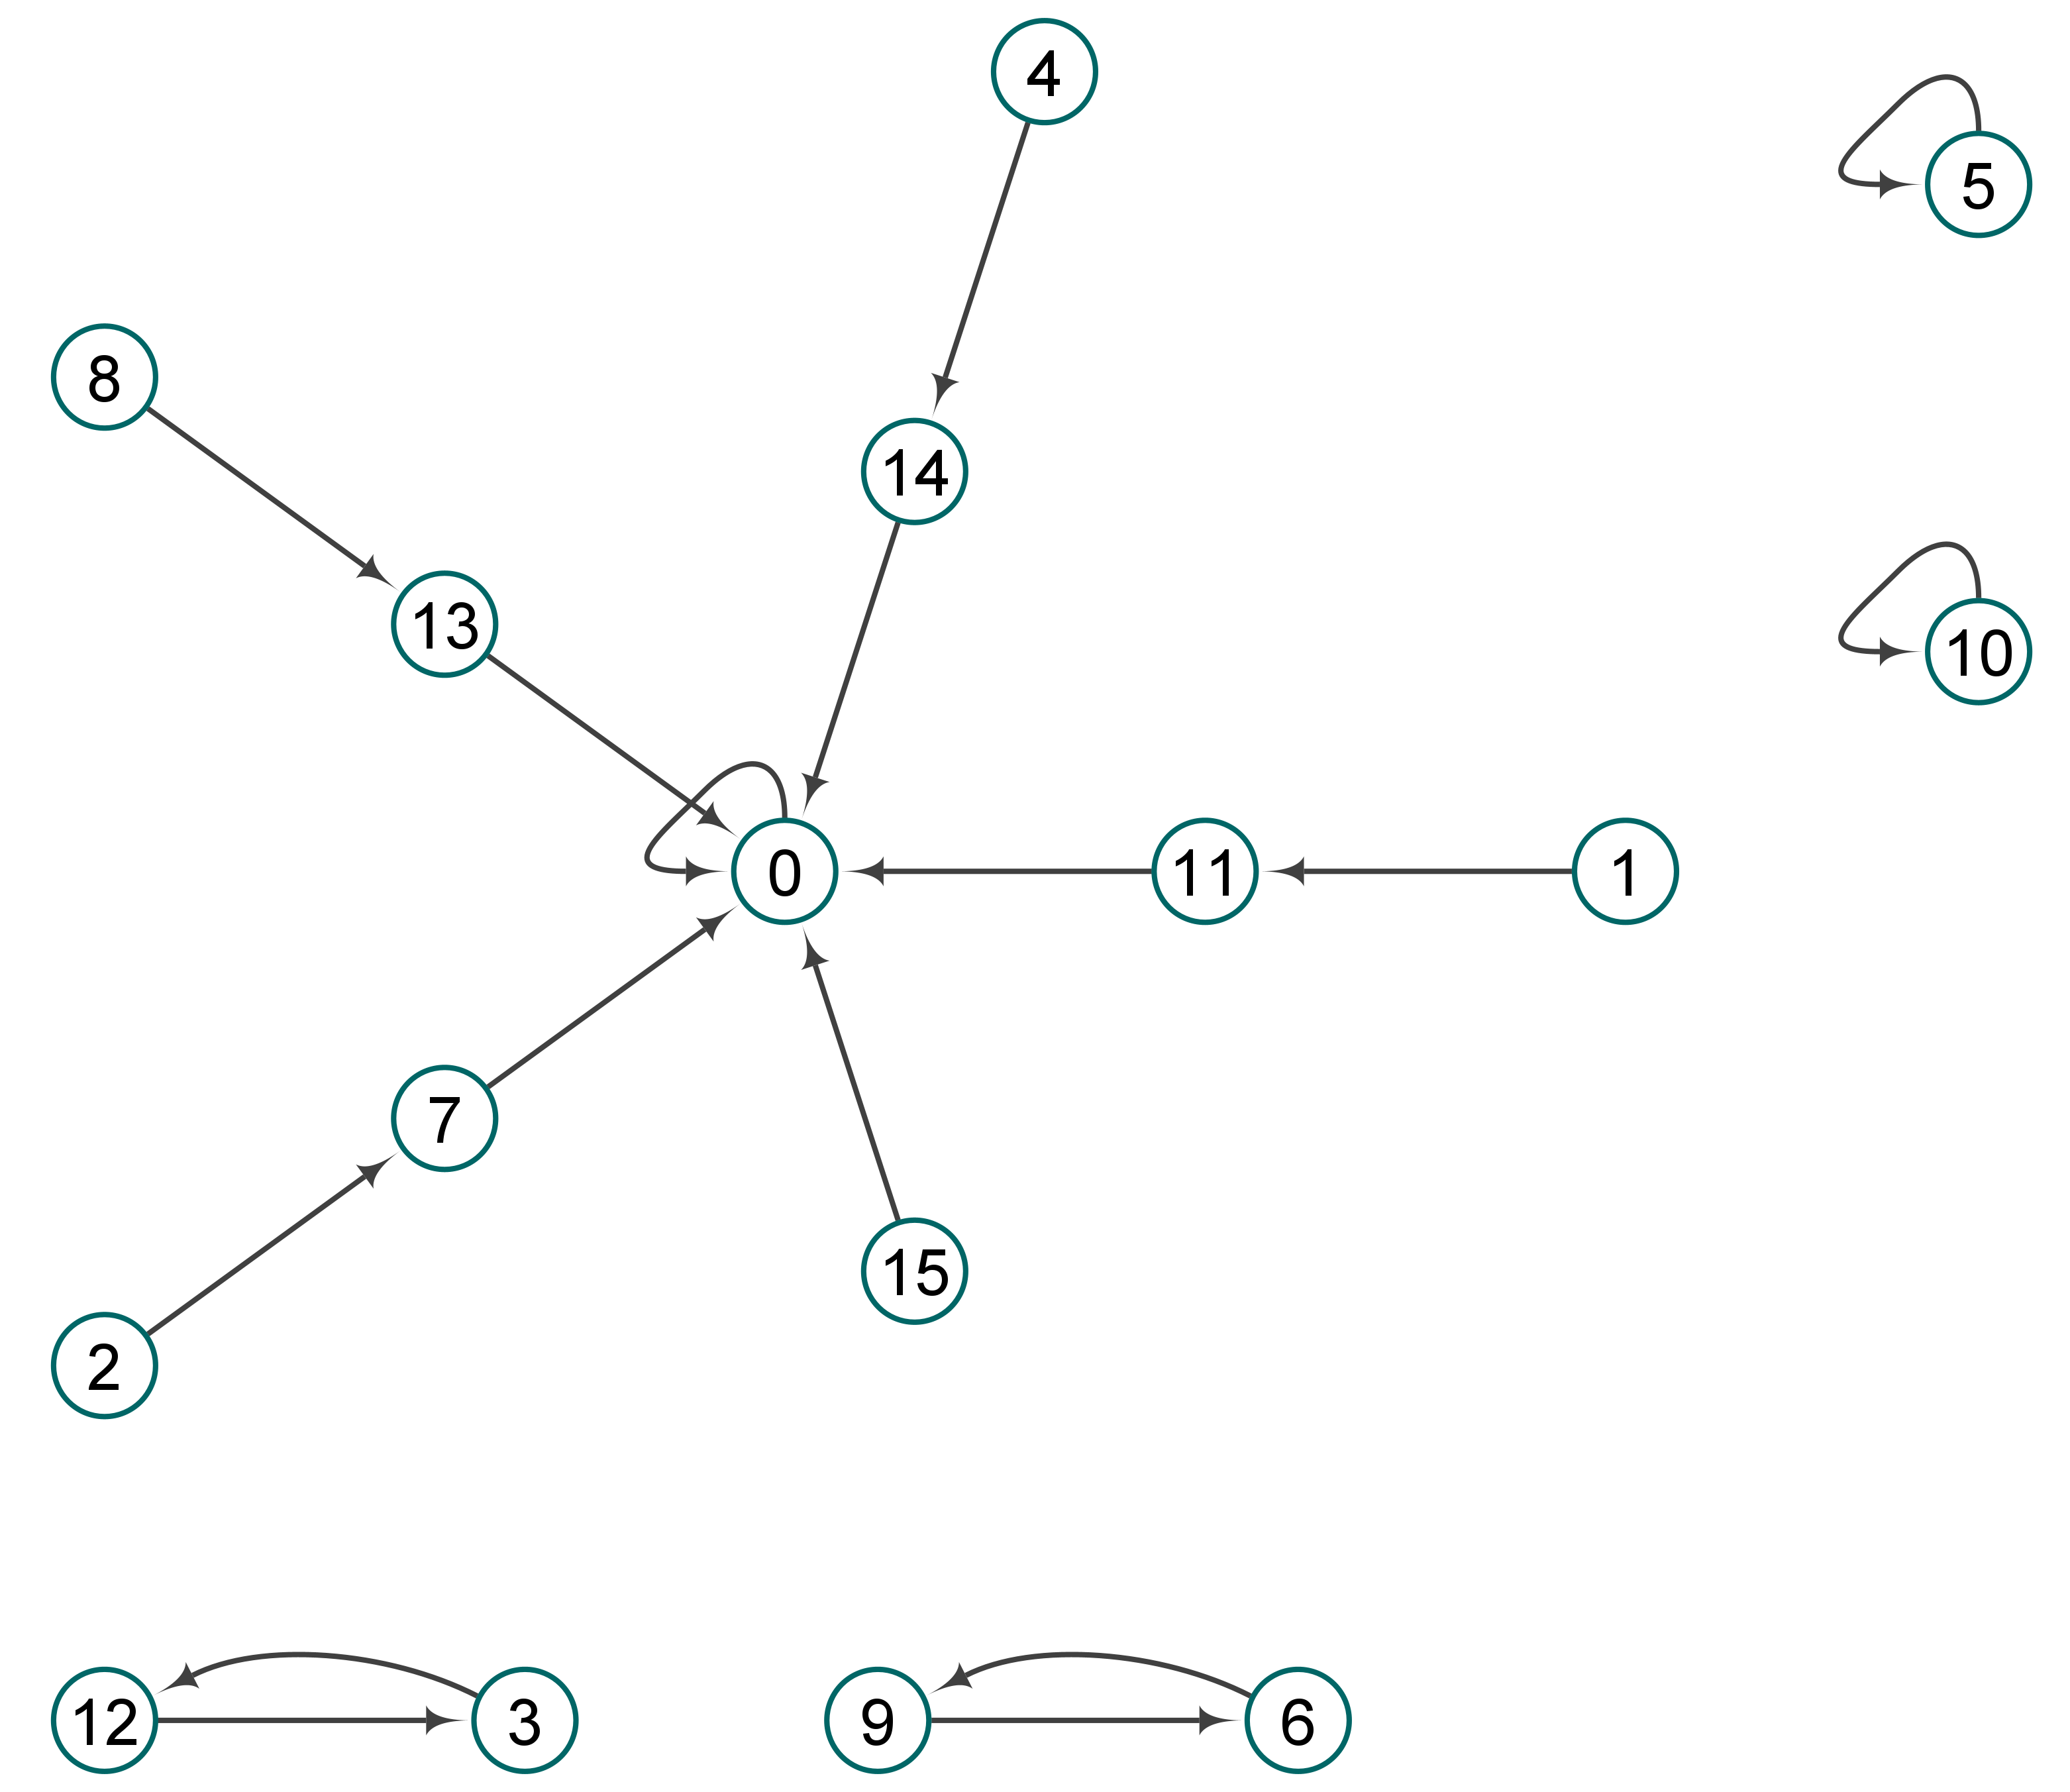
\includegraphics[scale=0.1]{resources/Atractores22/atractor_22_size_4.png}
			\caption{Atractor de tamaño 4.}\label{fig:picture}
			\end{figure}
			\begin{figure}[H]
			\centering
			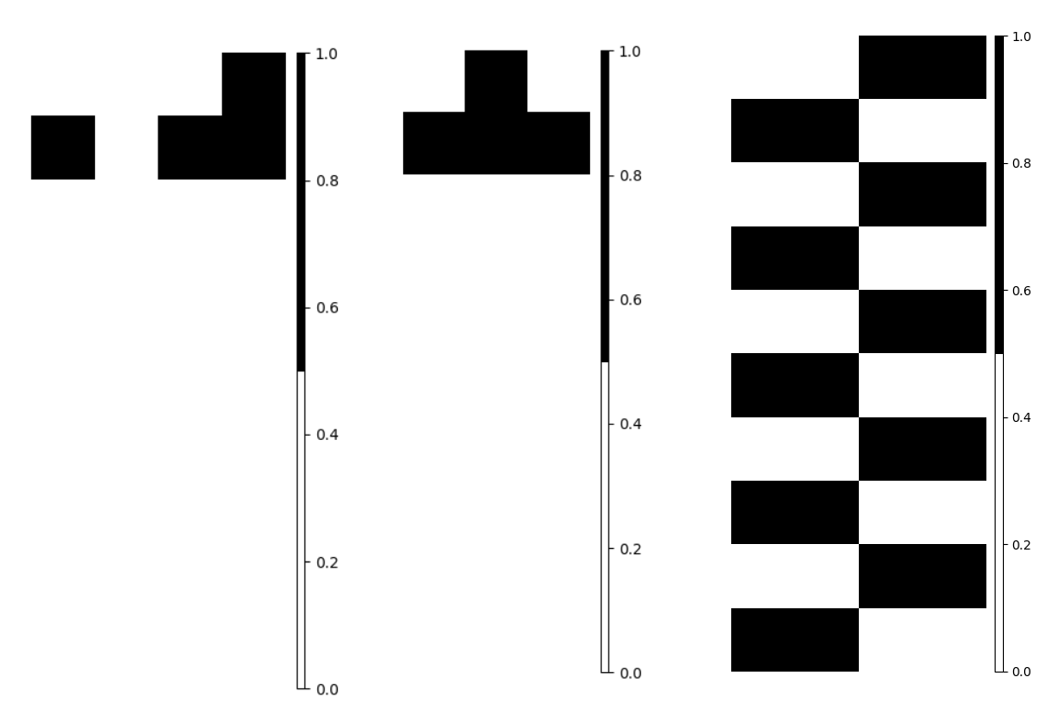
\includegraphics[scale=0.3]{resources/Atractores22/atractor_22_size_4_res.png}
			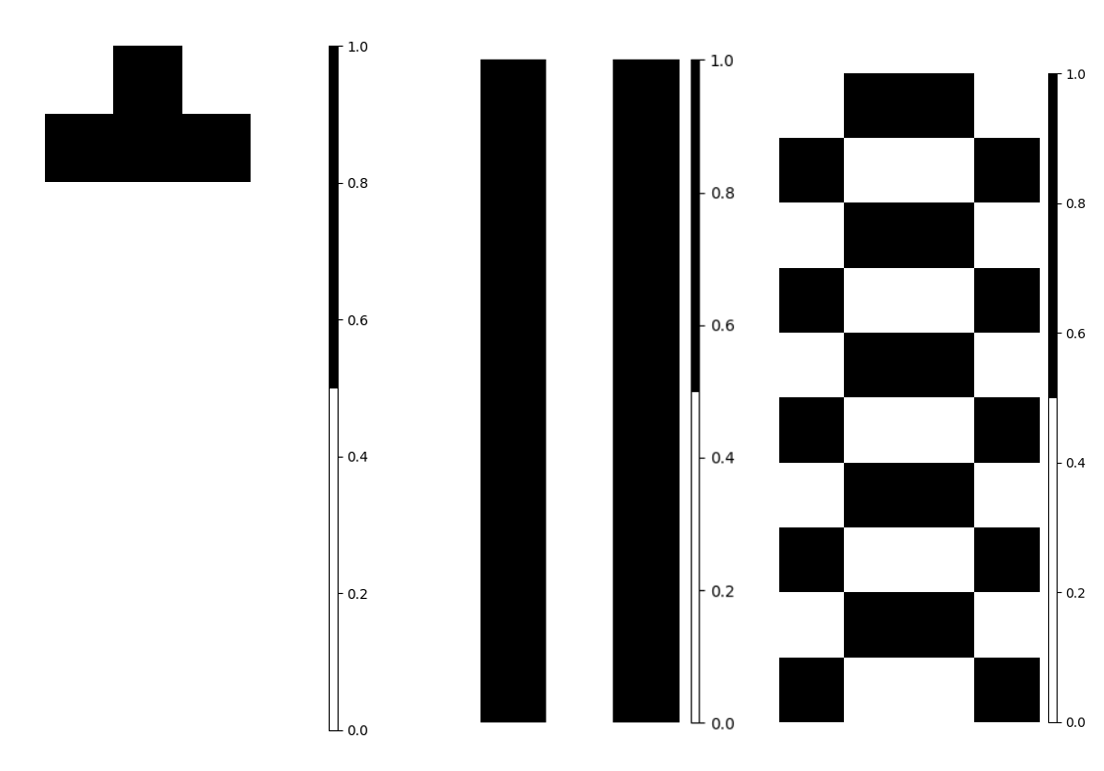
\includegraphics[scale=0.3]{resources/Atractores22/atractor_22_size_4_res1.png}
			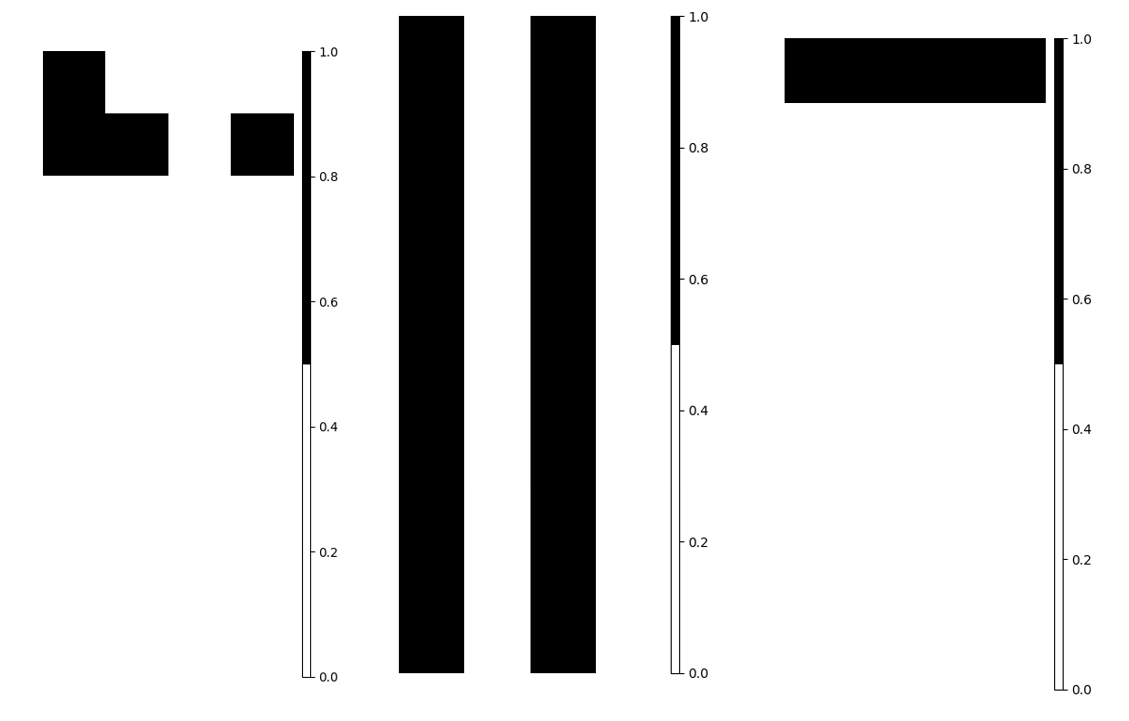
\includegraphics[scale=0.3]{resources/Atractores22/atractor_22_size_4_res2.png}
			\caption{Evoluciones de los atractores.}\label{fig:picture}
			\end{figure}
			Mencionar que para este atractor no vemos el caso del nodo 0, 13, 14, 7, 12 y 9 ya se pueden ver sus evoluciones por medio de otros nodos, por ejemplo, para ver la evolución del nodo 12 hacemos uso del nodo 3 ya que es un ciclo entre ambos, en el caso del nodo 9 y 6 ocurre lo mismo, mientras que los nodos 8, 4, 1, 2 y 15 acceden al nodo 0, los 4 primeros pasan por otros nodos, los cuales son 13, 14, 11 y 7 respectivamente.
			\subsubsection{Tamaño 5}
			\begin{figure}[H]
			\centering
			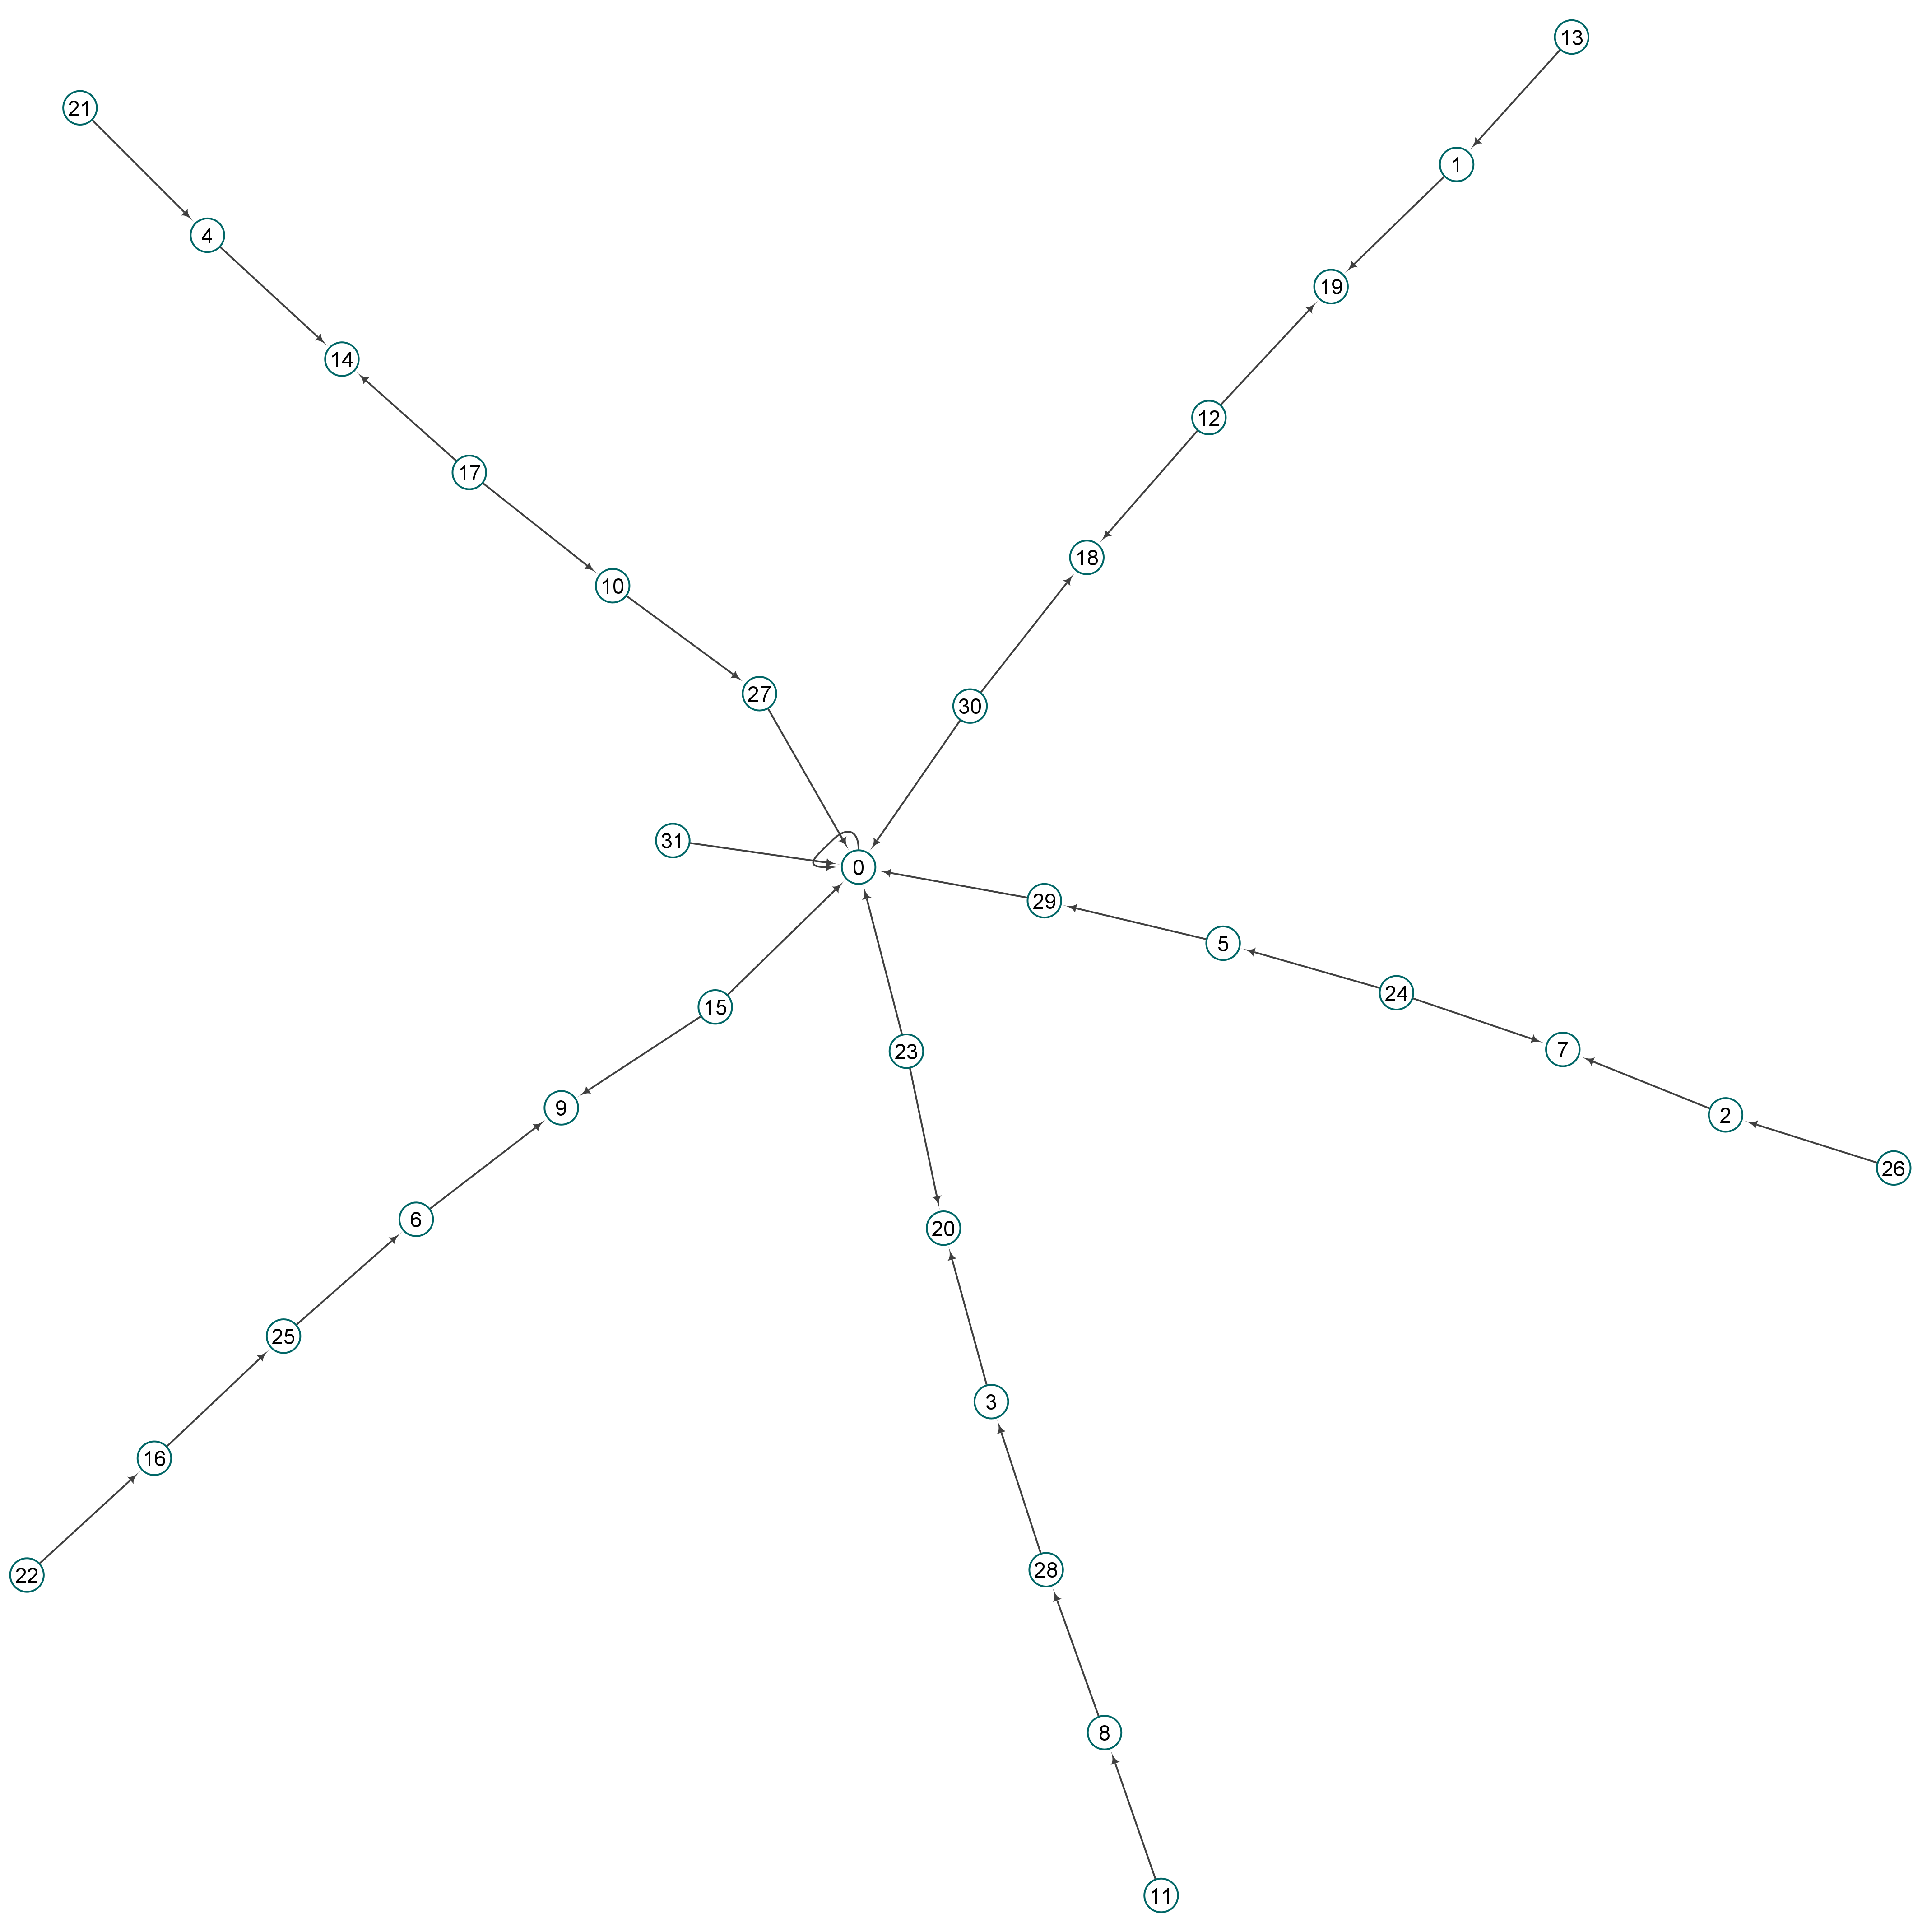
\includegraphics[scale=0.1]{resources/Atractores22/atractor_22_size_5.png}
			\caption{Atractor de tamaño 5.}\label{fig:picture}
			\end{figure}
			\begin{figure}[H]
			\centering
			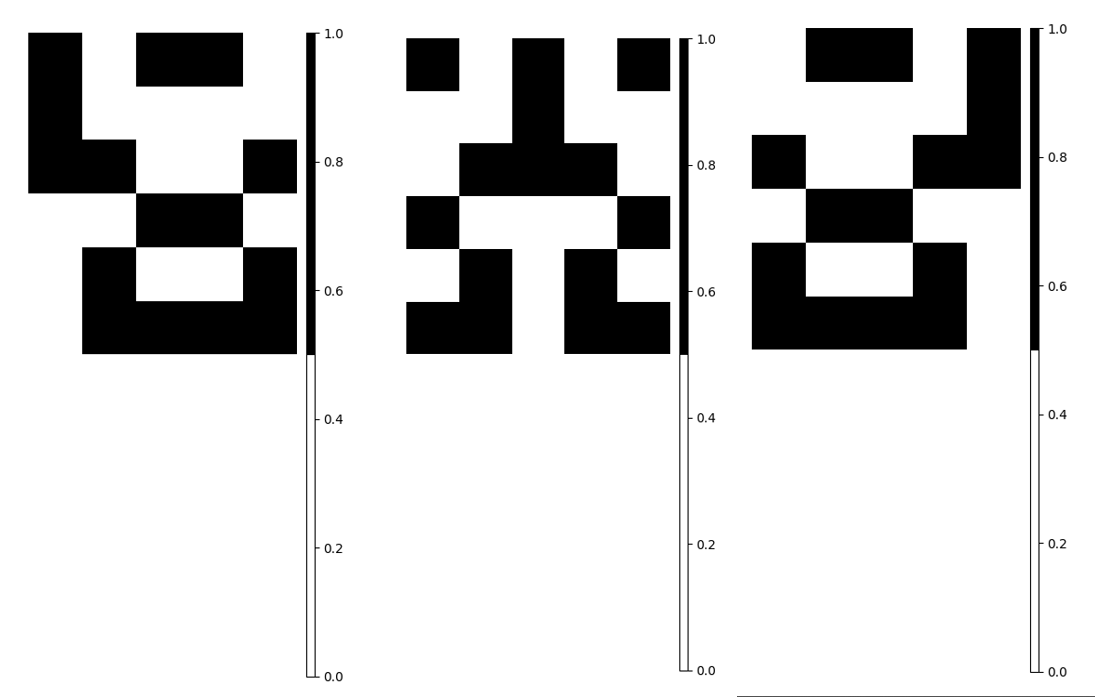
\includegraphics[scale=0.3]{resources/Atractores22/atractor_22_size_5_res.png}
			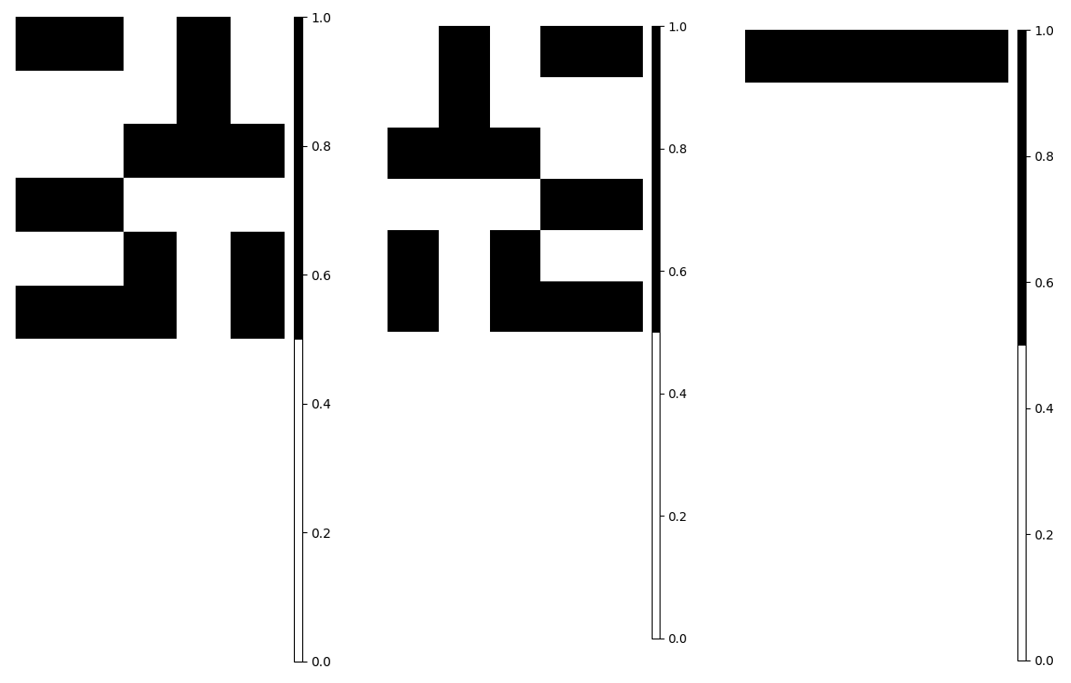
\includegraphics[scale=0.3]{resources/Atractores22/atractor_22_size_5_res1.png}
			\caption{Evoluciones de los atractores.}\label{fig:picture}
			\end{figure}
			Mencionar que para este atractor solamente vemos la evolución de los nodos 11, 22, 31, 21, 13 y 26, ya que son los nodos del exterior y estos pasan por los demás nodos y podemos ver como funciona el atractor el cual es el nodo 0.
			\subsubsection{Tamaño 6}
			\begin{figure}[H]
			\centering
			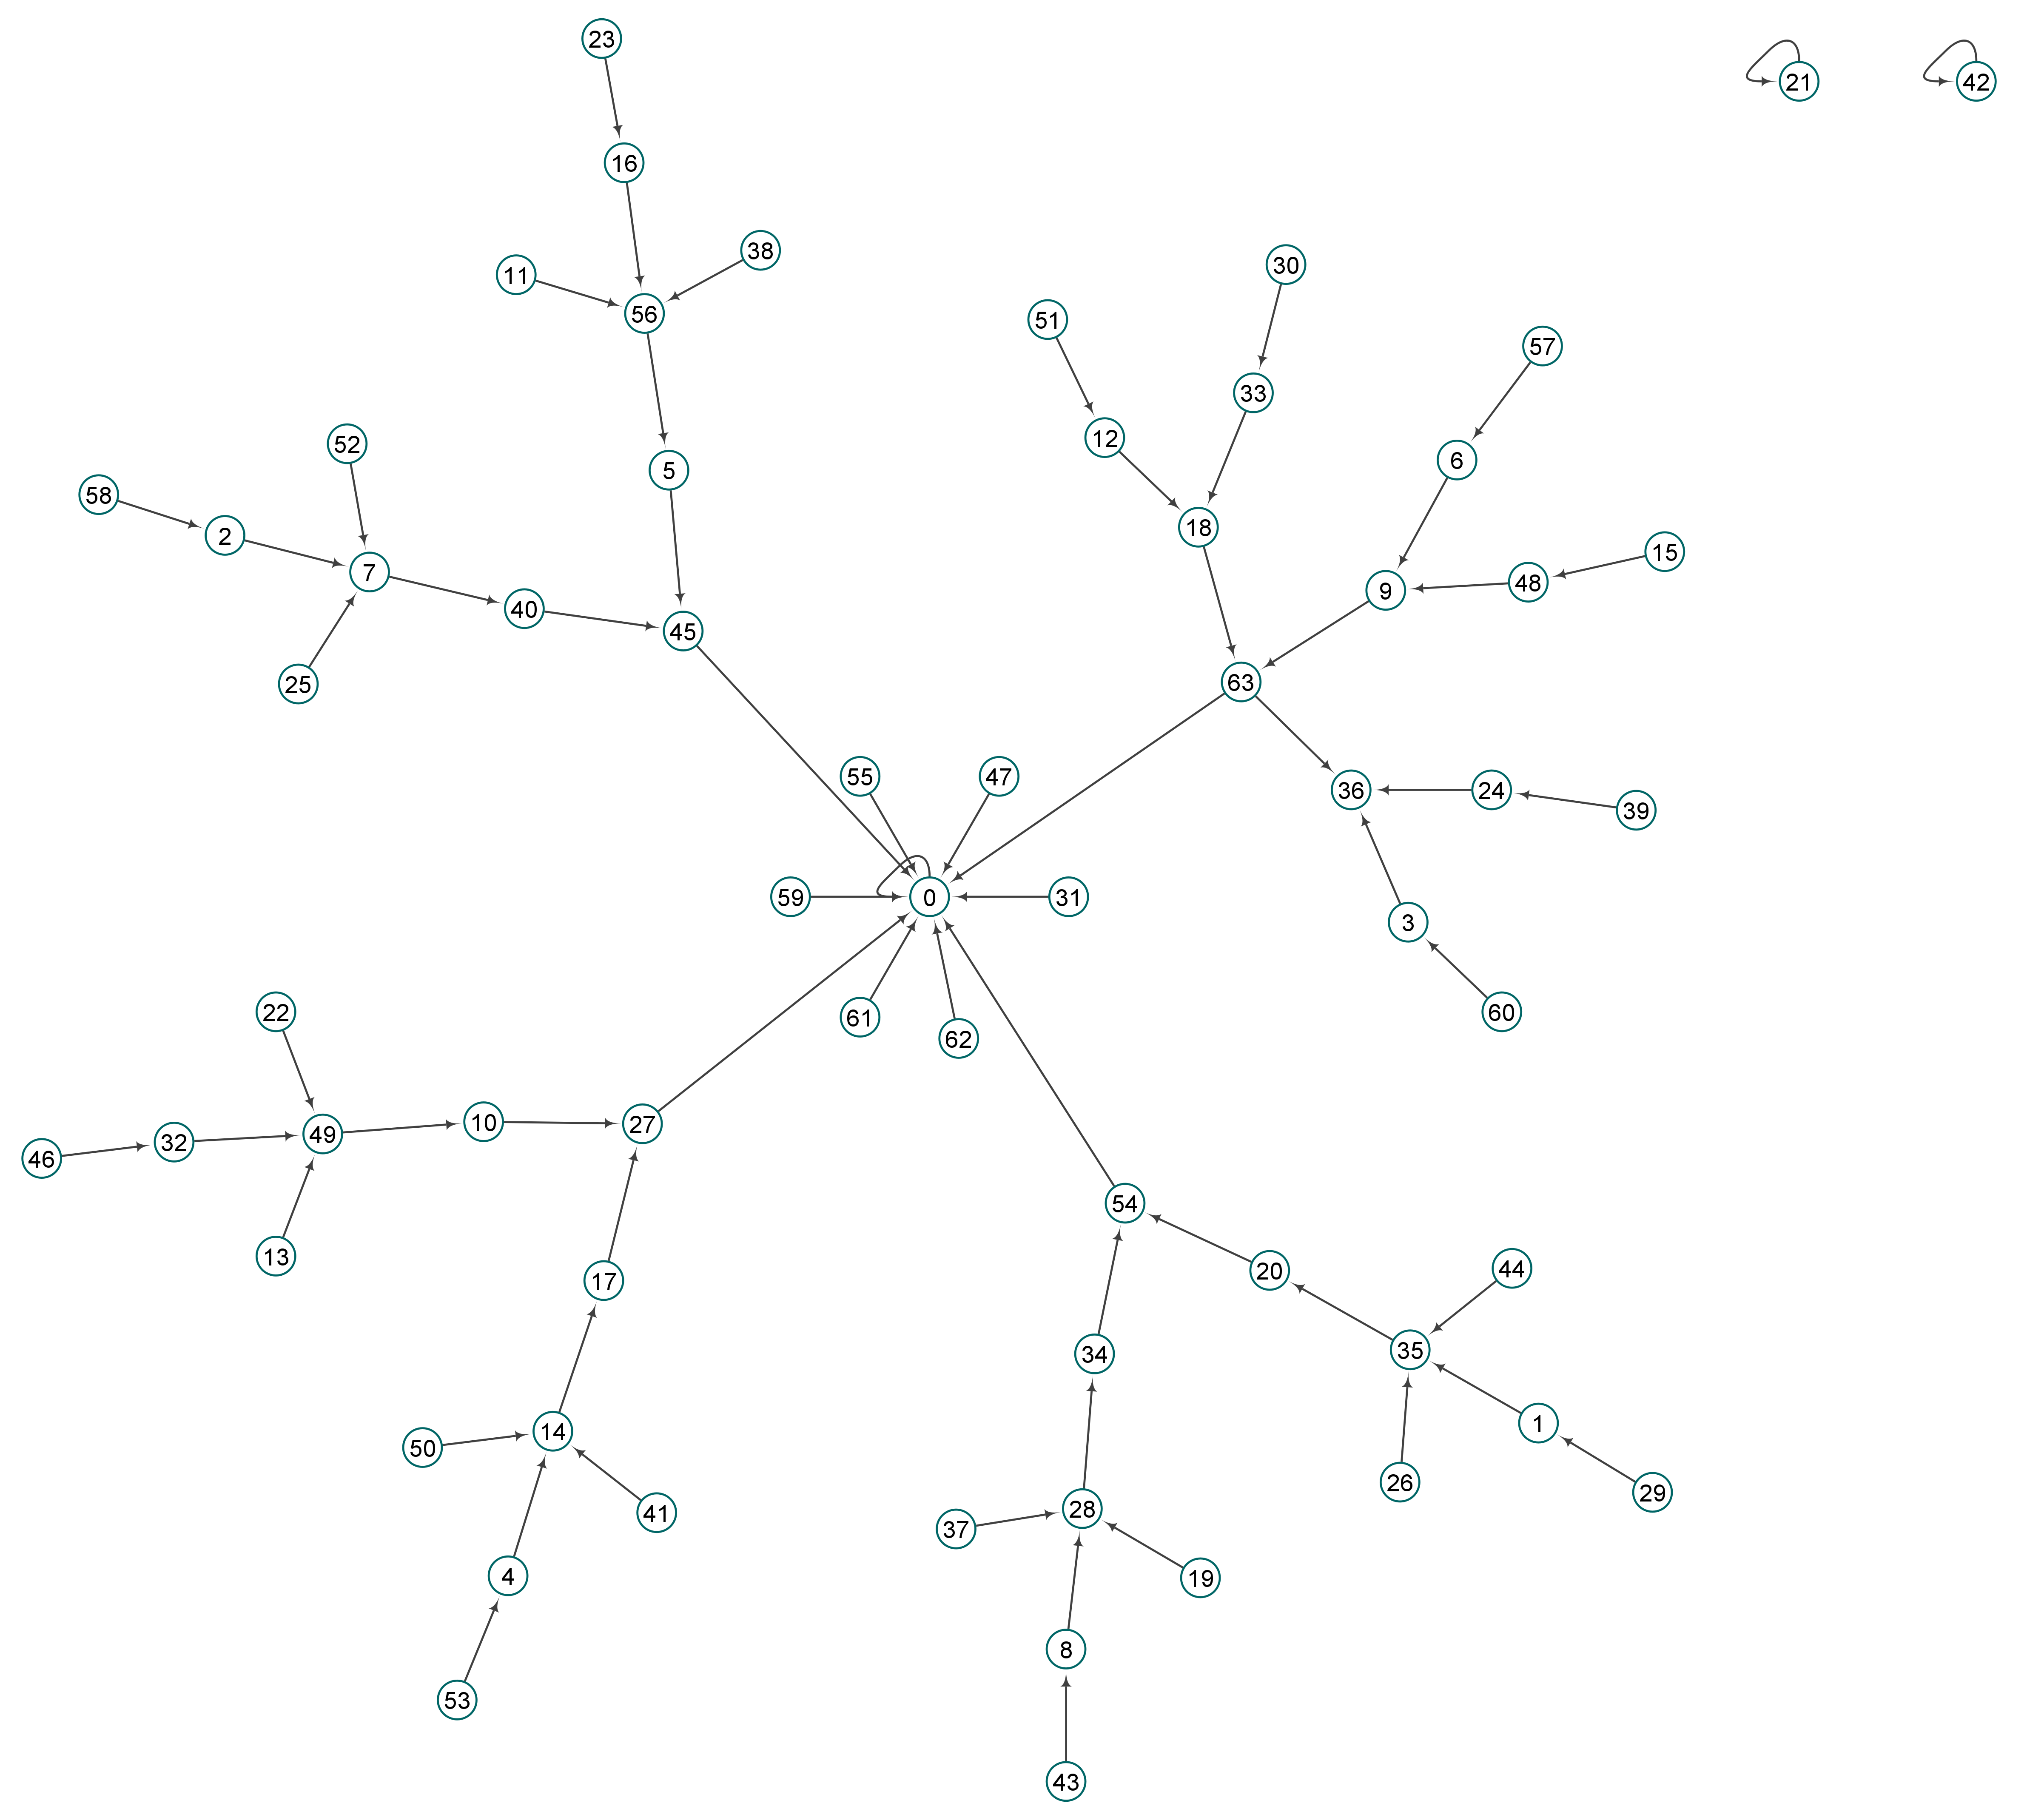
\includegraphics[scale=0.1]{resources/Atractores22/atractor_22_size_6.png}
			\caption{Atractor de tamaño 6.}\label{fig:picture}
			\end{figure}
			\begin{figure}[H]
			\centering
			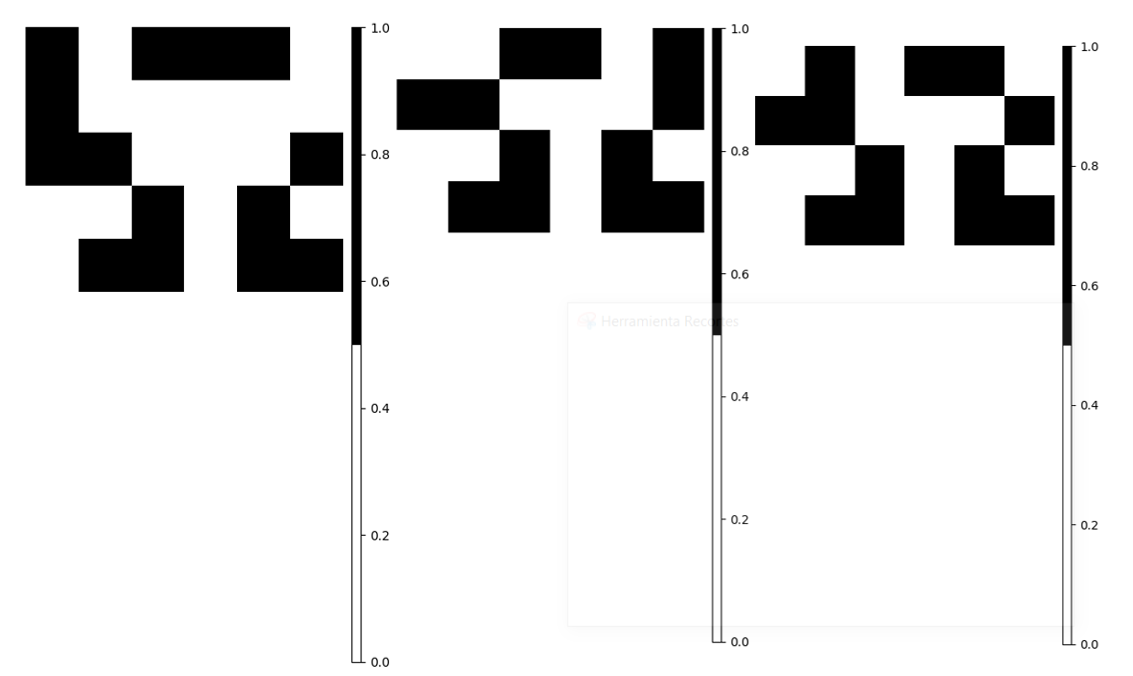
\includegraphics[scale=0.3]{resources/Atractores22/atractor_22_size_6_res.png}
			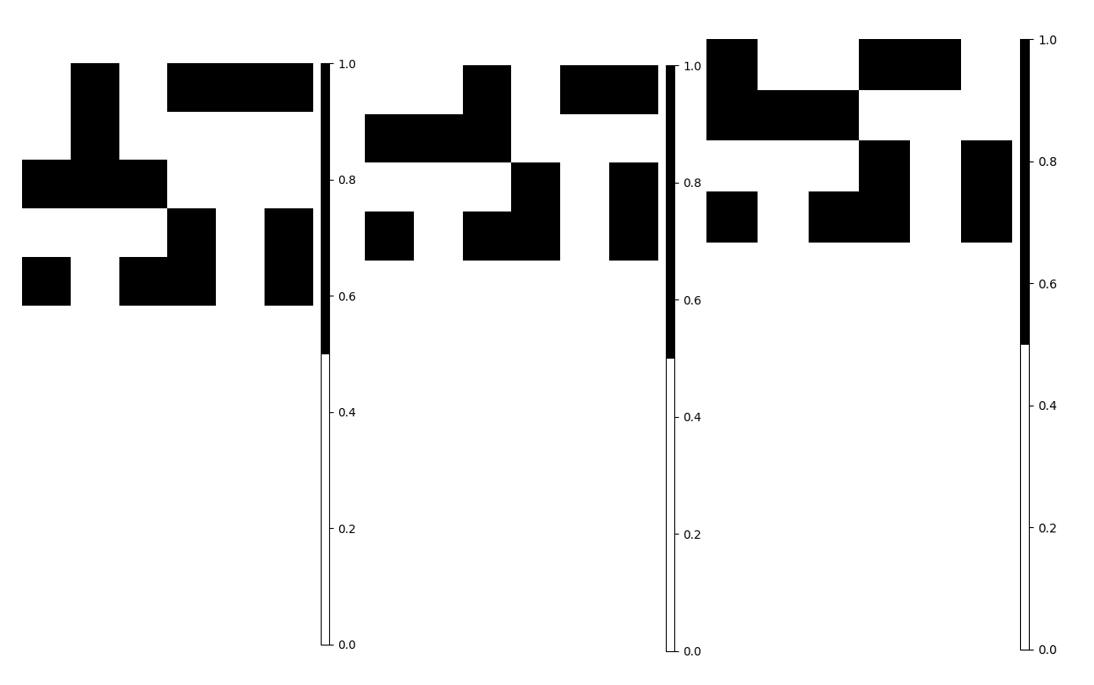
\includegraphics[scale=0.3]{resources/Atractores22/atractor_22_size_6_res2.png}
			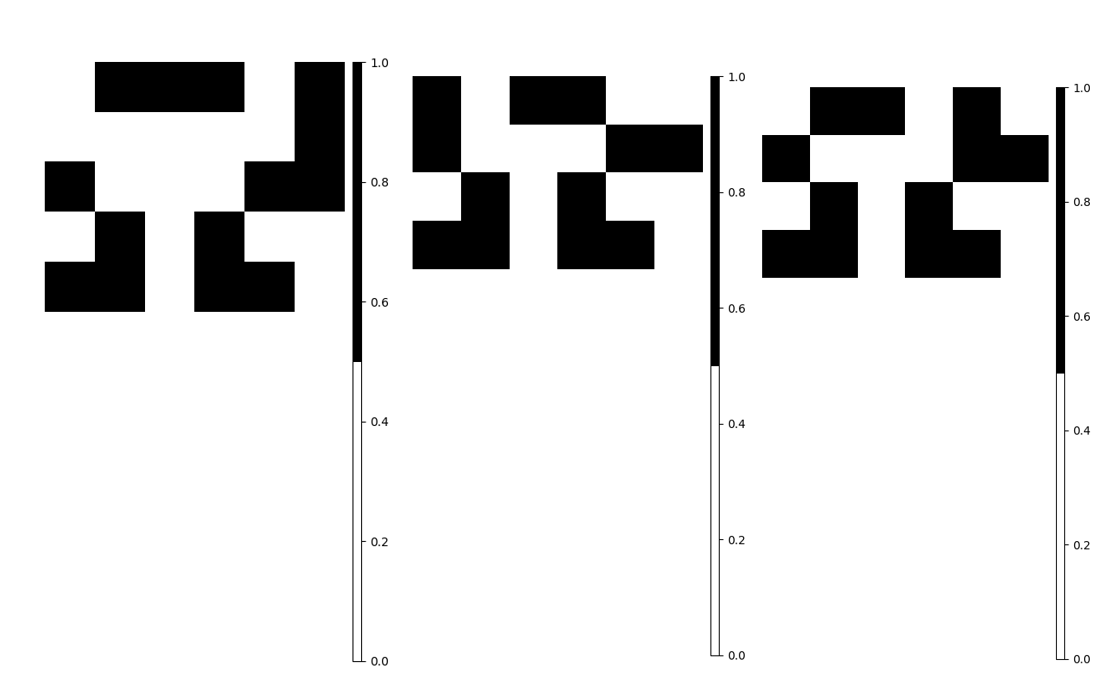
\includegraphics[scale=0.3]{resources/Atractores22/atractor_22_size_6_res5.png}
			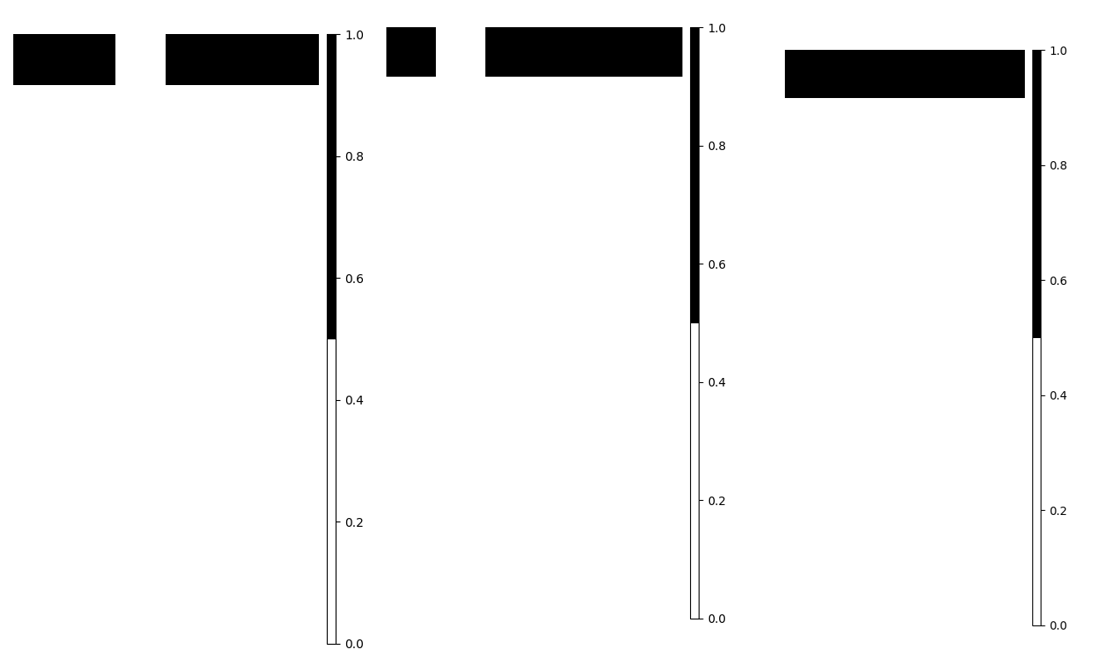
\includegraphics[scale=0.3]{resources/Atractores22/atractor_22_size_6_res9.png}
			\caption{Evoluciones de los atractores.}\label{fig:picture}
			\end{figure}
			Mencionar que a partir de este atractor solamente tomaremos unos cuantos nodos de prueba ya que abarcar la mayoría tomaría mucho espacio del reporte.
			\subsubsection{Tamaño 7}
			\begin{figure}[H]
			\centering
			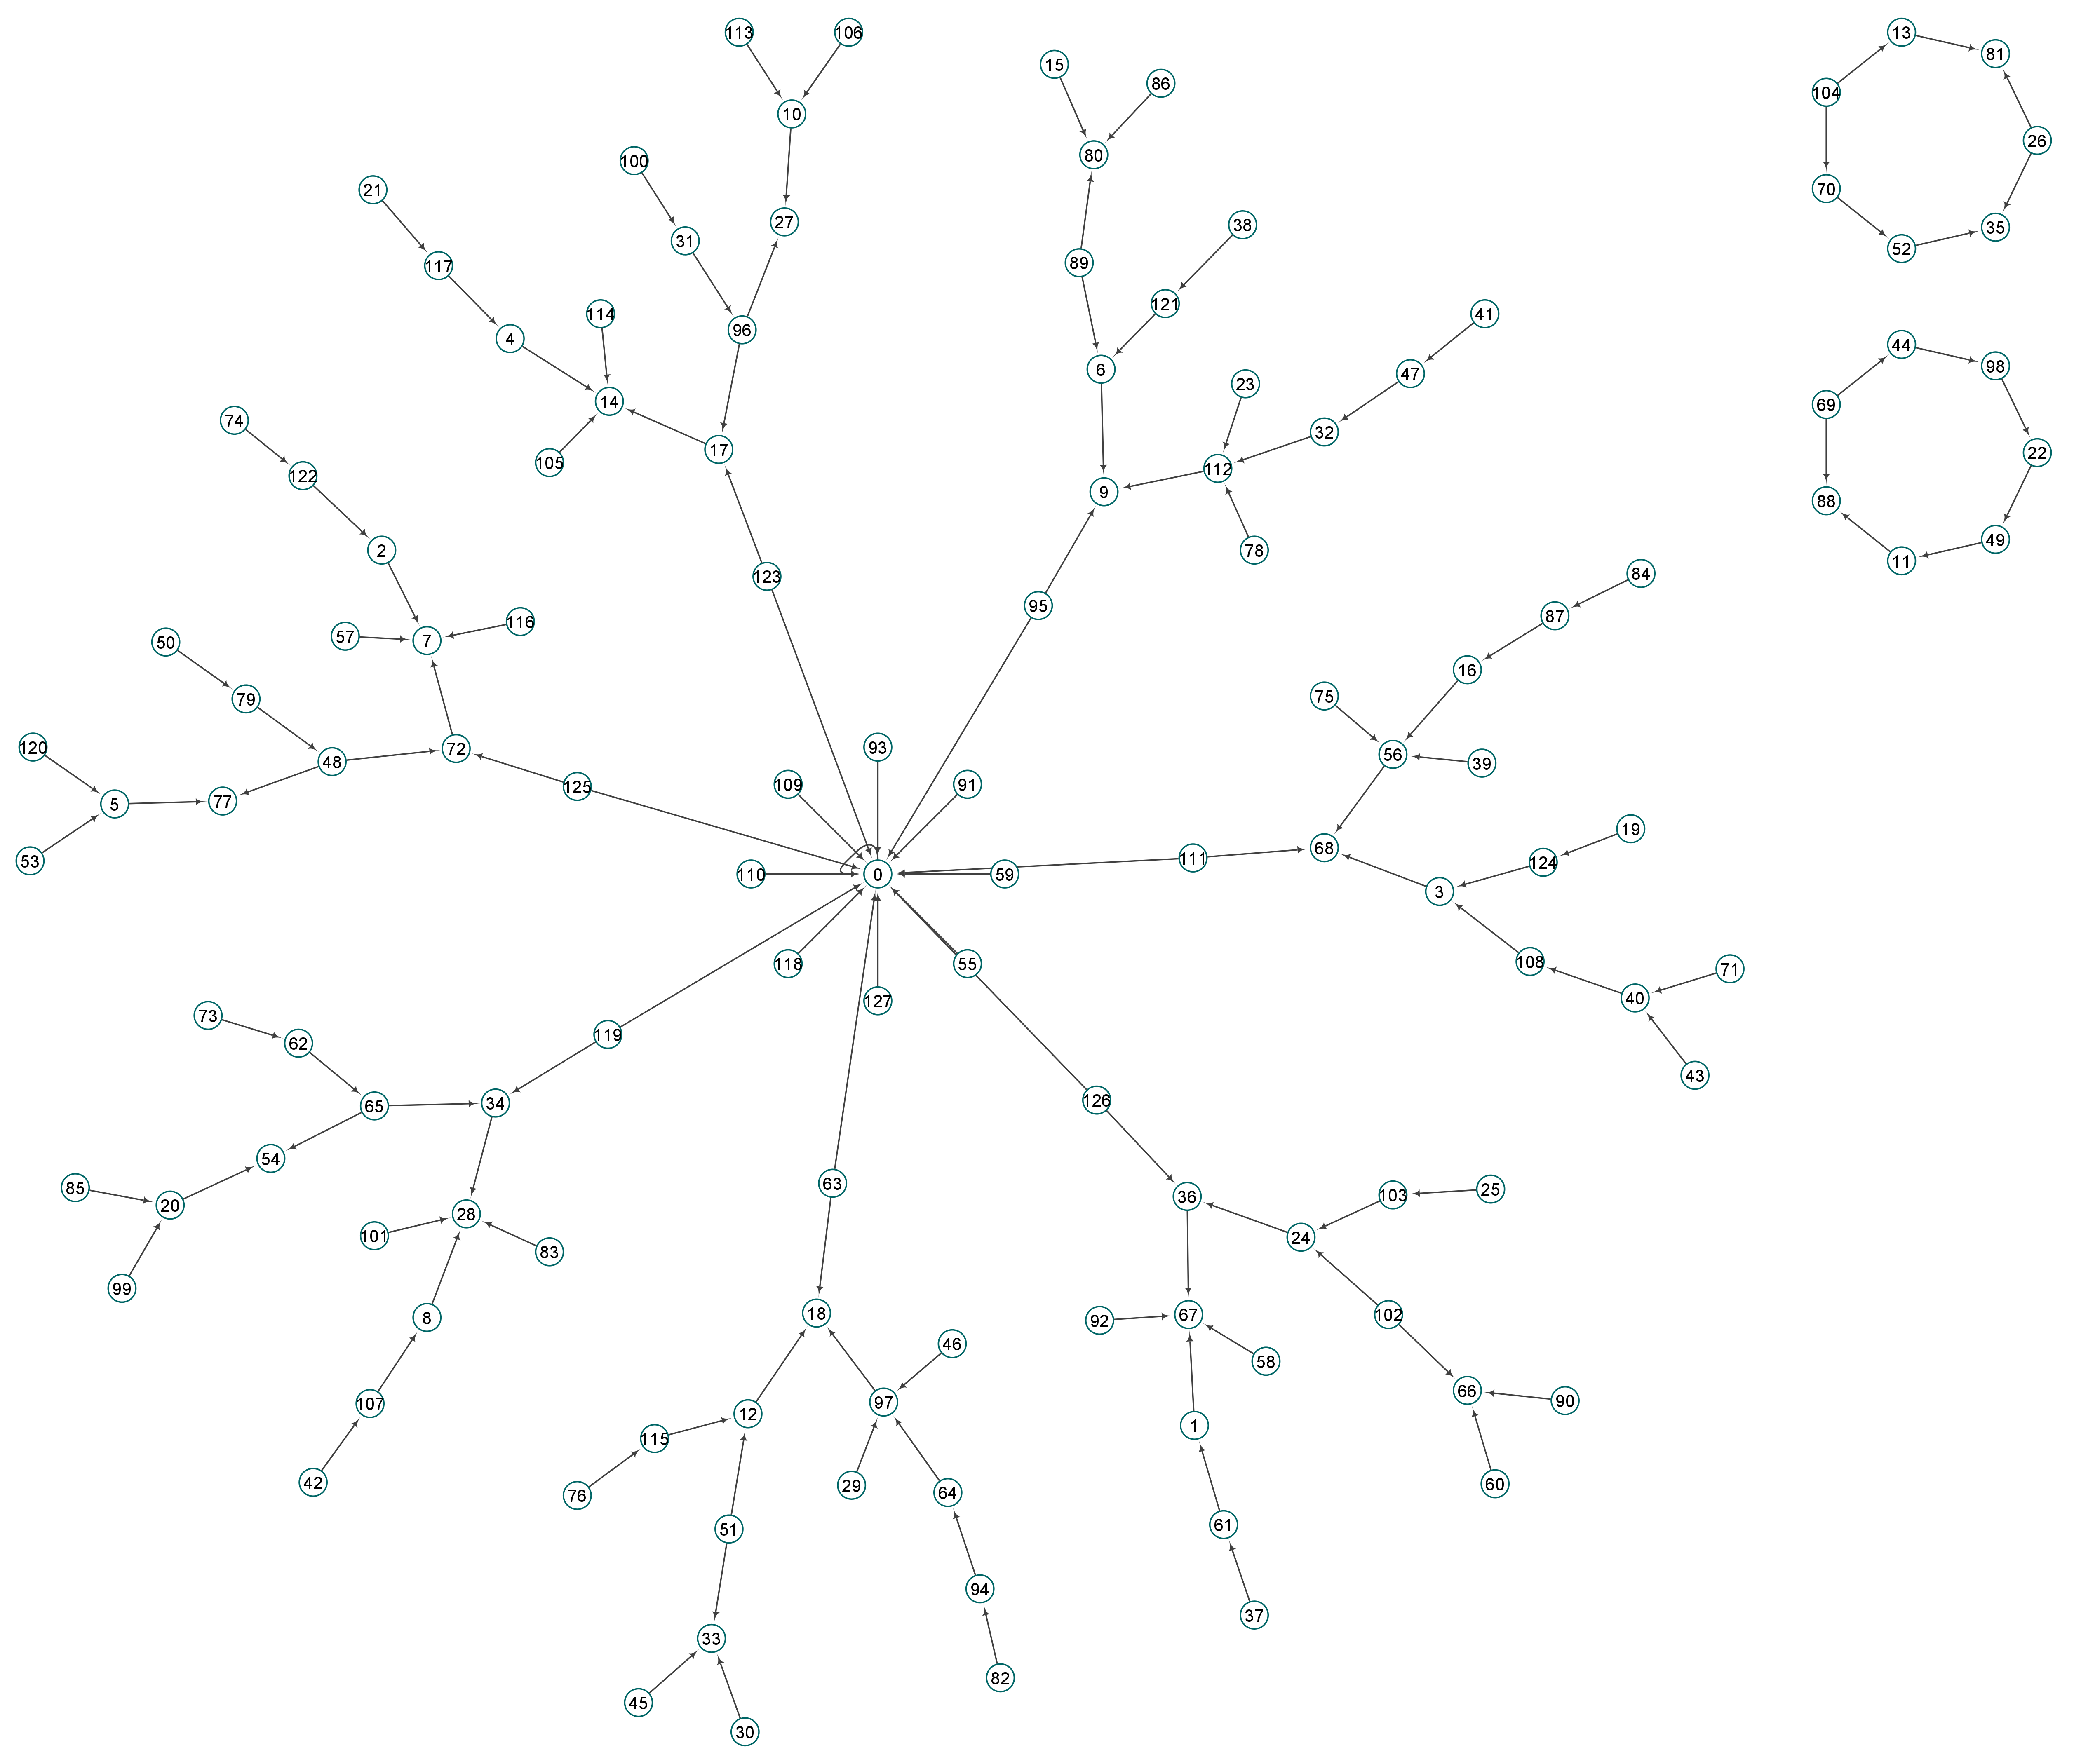
\includegraphics[scale=0.1]{resources/Atractores22/atractor_22_size_7.png}
			\caption{Atractor de tamaño 7.}\label{fig:picture}
			\end{figure}
			\begin{figure}[H]
			\centering
			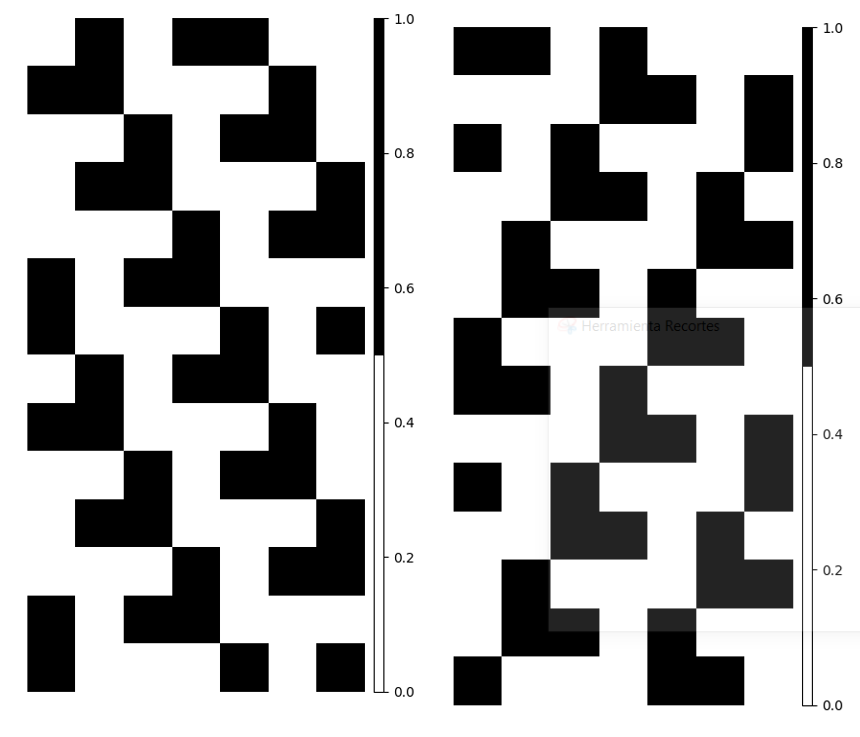
\includegraphics[scale=0.3]{resources/Atractores22/atractor_22_size_7_res.png}
			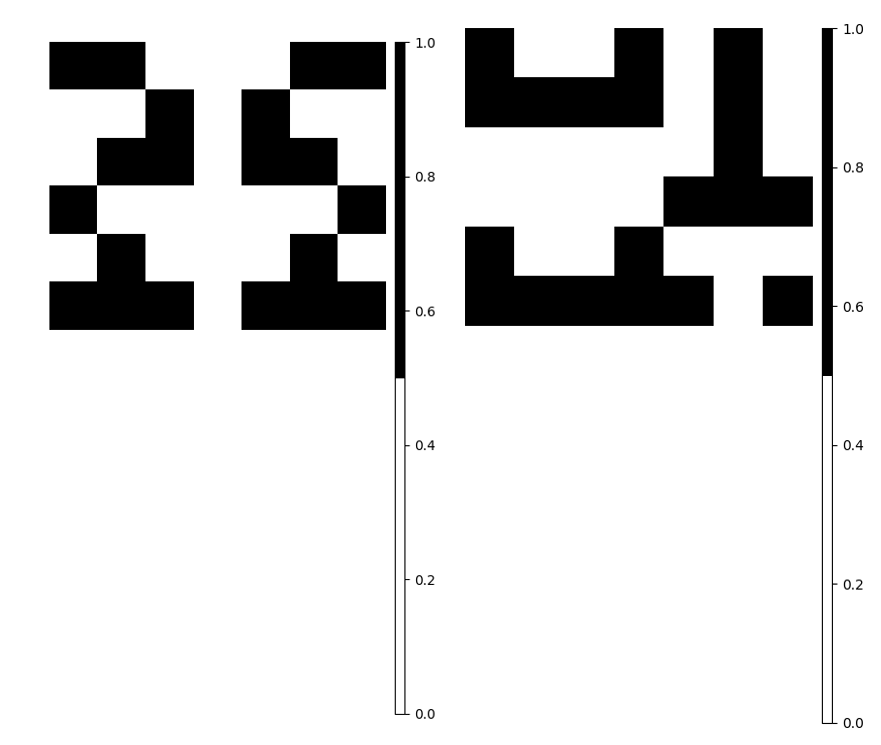
\includegraphics[scale=0.3]{resources/Atractores22/atractor_22_size_7_res1.png}
			\caption{Evoluciones de los atractores.}\label{fig:picture}
			\end{figure}
			Los nodos de prueba fueron 104, 44, 99 y 73, ya que empezamos a ver un patron repetitivo de tener nodos que se dirigen directamente al atractor y algunos nodos que forman ciclos con otros nodos.
			\subsubsection{Tamaño 8}
			\begin{figure}[H]
			\centering
			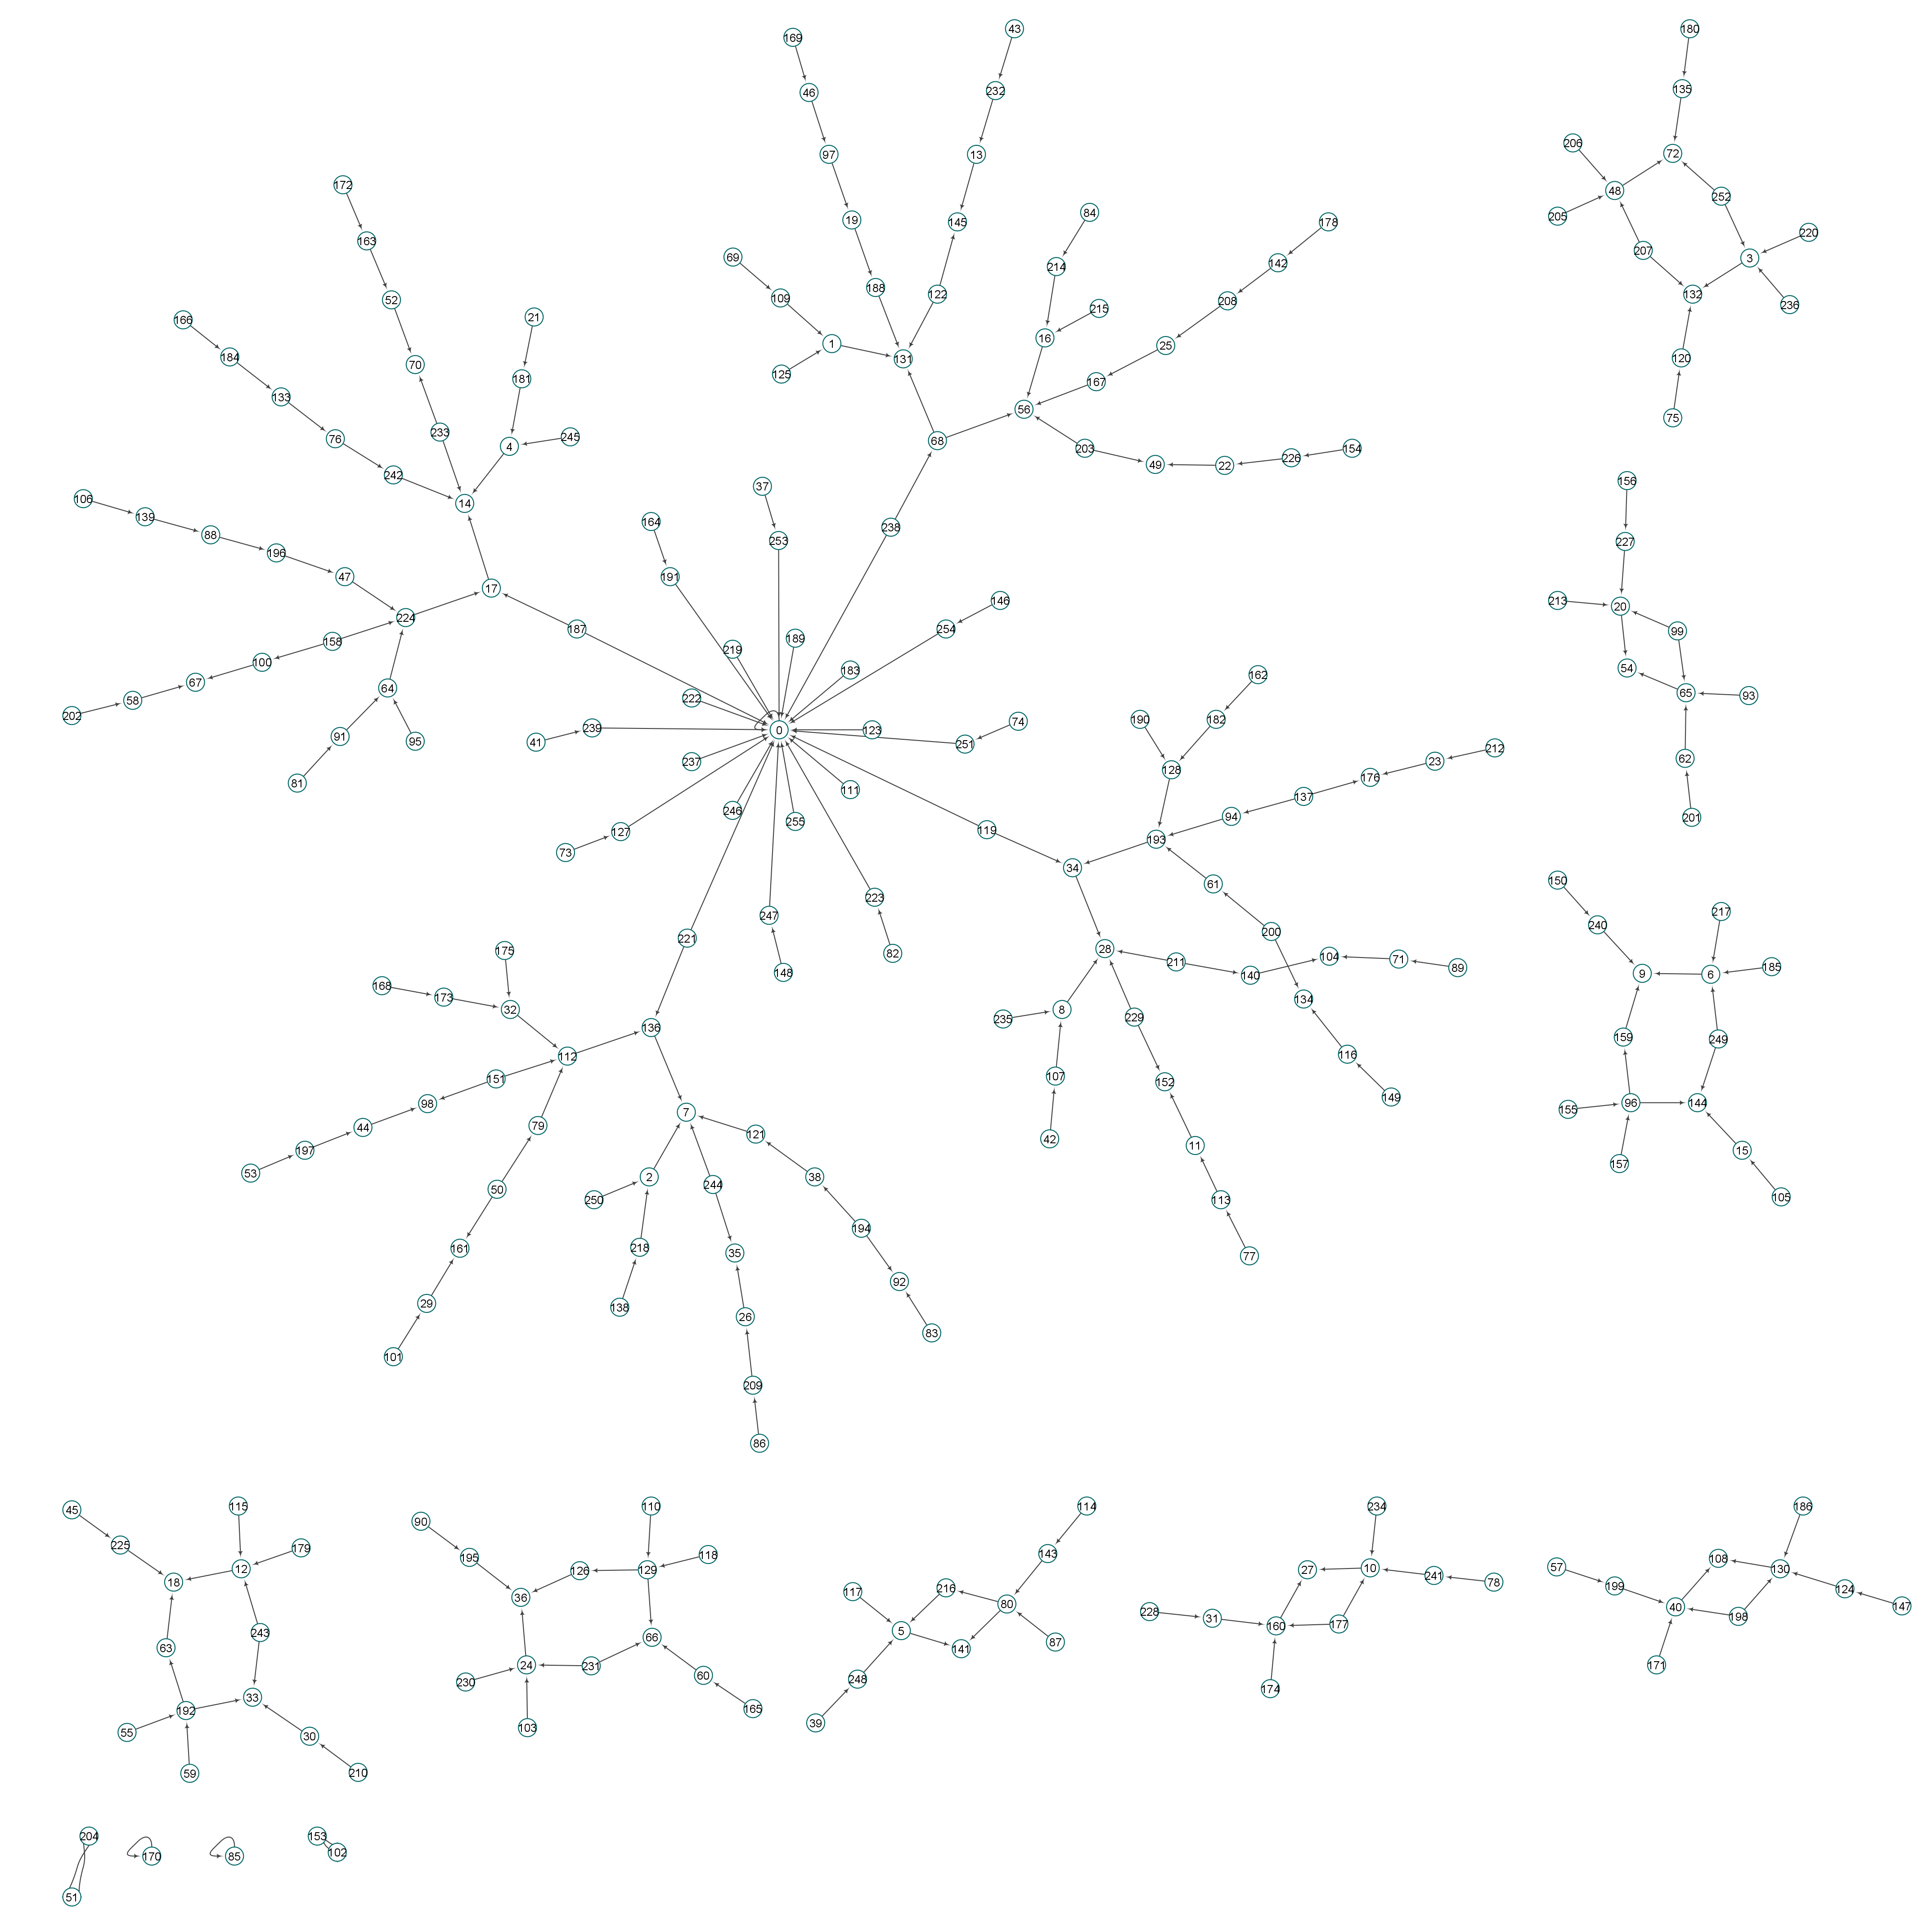
\includegraphics[scale=0.1]{resources/Atractores22/atractor_22_size_8.png}
			\caption{Atractor de tamaño 8.}\label{fig:picture}
			\end{figure}
			\begin{figure}[H]
			\centering
			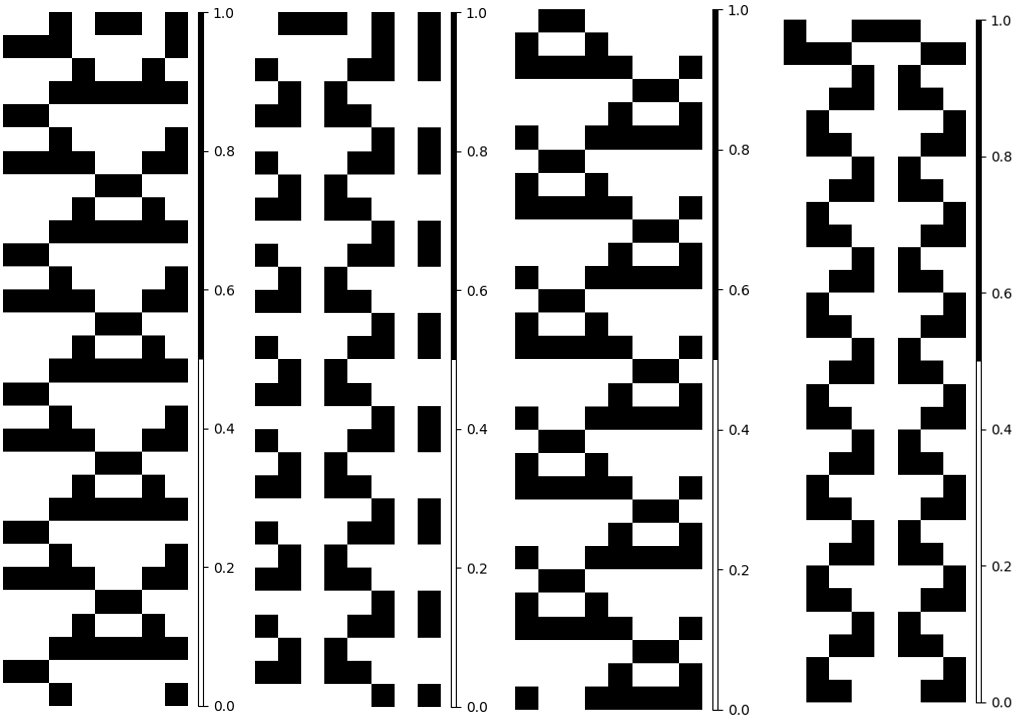
\includegraphics[scale=0.3]{resources/Atractores22/atractor_22_size_8_res.png}
			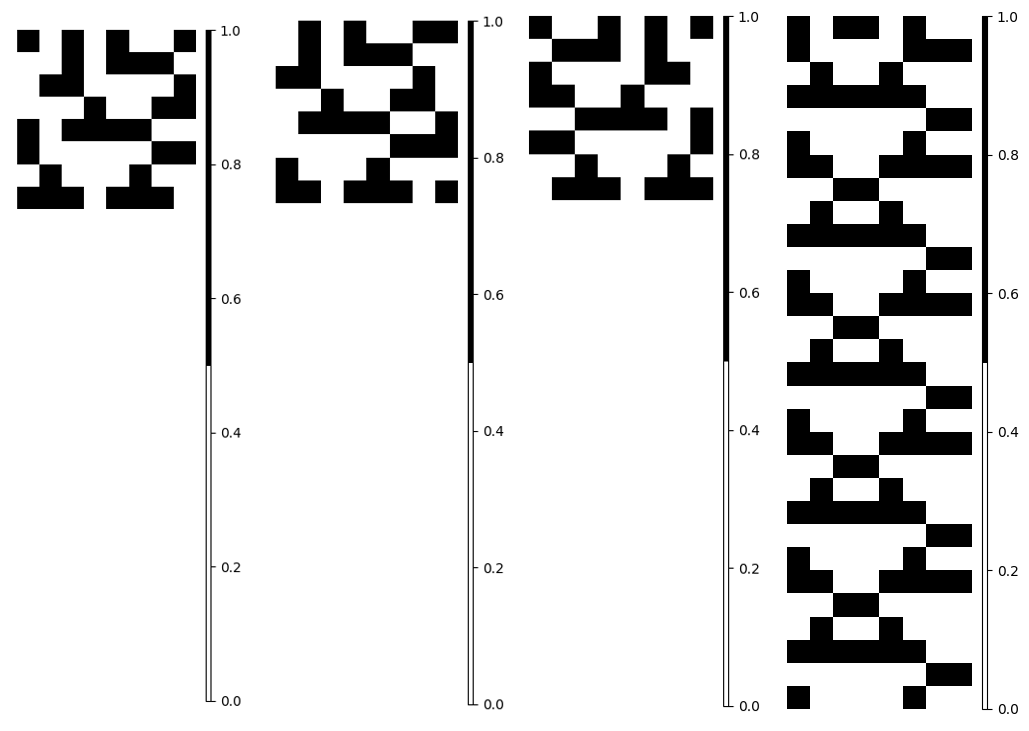
\includegraphics[scale=0.3]{resources/Atractores22/atractor_22_size_8_res1.png}
			\caption{Evoluciones de algunos atractores.}\label{fig:picture}
			\end{figure}
			\subsubsection{Tamaño 9}
			\begin{figure}[H]
			\centering
			\includegraphics[scale=0.1]{resources/Atractores22/atractor_22_size_9.png}
			\caption{Atractor de tamaño 9.}\label{fig:picture}
			\end{figure}
			\begin{figure}[H]
			\centering
			\includegraphics[scale=0.3]{resources/Atractores22/atractor_22_size_9_res.png}
			\includegraphics[scale=0.3]{resources/Atractores22/atractor_22_size_9_res1.png}
			\includegraphics[scale=0.3]{resources/Atractores22/atractor_22_size_9_res2.png}
			\caption{Evoluciones de los atractores.}\label{fig:picture}
			\end{figure}
			\subsubsection{Tamaño 10}
			\begin{figure}[H]
			\centering
			\includegraphics[scale=0.1]{resources/Atractores22/atractor_22_size_10.png}
			\caption{Atractor de tamaño 10.}\label{fig:picture}
			\end{figure}
			\begin{figure}[H]
			\centering
			\includegraphics[scale=0.3]{resources/Atractores22/atractor_22_size_10_res.png}
			\includegraphics[scale=0.3]{resources/Atractores22/atractor_22_size_10_res1.png}
			\caption{Evoluciones de los atractores.}\label{fig:picture}
			\end{figure}
			\subsubsection{Tamaño 11}
			\begin{figure}[H]
			\centering
			\includegraphics[scale=0.1]{resources/Atractores22/atractor_22_size_11.png}
			\caption{Atractor de tamaño 11.}\label{fig:picture}
			\end{figure}
			\begin{figure}[H]
			\centering
			\includegraphics[scale=0.3]{resources/Atractores22/atractor_22_size_11_res.png}
			\includegraphics[scale=0.3]{resources/Atractores22/atractor_22_size_11_res1.png}
			\caption{Evoluciones de los atractores.}\label{fig:picture}
			\end{figure}
			\subsubsection{Tamaño 12}
			\begin{figure}[H]
			\centering
			\includegraphics[scale=0.1]{resources/Atractores22/atractor_22_size_12.png}
			\caption{Atractor de tamaño 12.}\label{fig:picture}
			\end{figure}
			\begin{figure}[H]
			\centering
			\includegraphics[scale=0.3]{resources/Atractores22/atractor_22_size_12_res.png}
			\includegraphics[scale=0.3]{resources/Atractores22/atractor_22_size_12_res1.png}
			\caption{Evoluciones de los atractores.}\label{fig:picture}
			\end{figure}
			\subsubsection{Tamaño 13}
			\begin{figure}[H]
			\centering
			\includegraphics[scale=0.15]{resources/Atractores22/atractor_22_size_13.png}
			\caption{Atractor de tamaño 13.}\label{fig:picture}
			\end{figure}
			\begin{figure}[H]
			\centering
			\includegraphics[scale=0.3]{resources/Atractores22/atractor_22_size_13_res.png}
			\includegraphics[scale=0.3]{resources/Atractores22/atractor_22_size_13_res1.png}
			\includegraphics[scale=0.3]{resources/Atractores22/atractor_22_size_13_res2.png}
			\caption{Evoluciones de los atractores.}\label{fig:picture}
			\end{figure}
			\subsubsection{Tamaño 14}
			\begin{figure}[H]
			\centering
			\includegraphics[scale=0.1]{resources/Atractores22/atractor_22_size_14.png}
			\caption{Atractor de tamaño 14.}\label{fig:picture}
			\end{figure}
			\begin{figure}[H]
			\centering
			\includegraphics[scale=0.3]{resources/Atractores22/atractor_22_size_14_res.png}
			\includegraphics[scale=0.3]{resources/Atractores22/atractor_22_size_14_res1.png}
			\includegraphics[scale=0.3]{resources/Atractores22/atractor_22_size_14_res2.png}
			\caption{Evoluciones de los atractores.}\label{fig:picture}
			\end{figure}
			\subsubsection{Tamaño 15}
			\begin{figure}[H]
			\centering
			\includegraphics[scale=0.8]{resources/Atractores22/atractor_22_size_15.png}
			\caption{Atractor de tamaño 15.}\label{fig:picture}
			\end{figure}
			\begin{figure}[H]
			\centering
			\includegraphics[scale=0.3]{resources/Atractores22/atractor_22_size_15_res.png}
			\includegraphics[scale=0.3]{resources/Atractores22/atractor_22_size_15_res1.png}
			\includegraphics[scale=0.3]{resources/Atractores22/atractor_22_size_15_res2.png}
			\caption{Evoluciones de los atractores.}\label{fig:picture}
			\end{figure}
			\subsubsection{Tamaño 16}
			\begin{figure}[H]
			\centering
			\includegraphics[scale=0.8]{resources/Atractores22/atractor_22_size_16.png}
			\caption{Atractor de tamaño 16.}\label{fig:picture}
			\end{figure}
			\begin{figure}[H]
			\centering
			\includegraphics[scale=0.3]{resources/Atractores22/atractor_22_size_16_res.png}
			\includegraphics[scale=0.3]{resources/Atractores22/atractor_22_size_16_res1.png}
			\includegraphics[scale=0.3]{resources/Atractores22/atractor_22_size_16_res2.png}
			\caption{Evoluciones de los atractores.}\label{fig:picture}
			\end{figure}
			\subsubsection{Tamaño 17}
			\begin{figure}[H]
			\centering
			\includegraphics[scale=0.7]{resources/Atractores22/atractor_22_size_17.png}
			\caption{Atractor de tamaño 17.}\label{fig:picture}
			\end{figure}
			\begin{figure}[H]
			\centering
			\includegraphics[scale=0.3]{resources/Atractores22/atractor_22_size_17_res.png}
			\includegraphics[scale=0.3]{resources/Atractores22/atractor_22_size_17_res1.png}
			\caption{Evoluciones de los atractores.}\label{fig:picture}
			\end{figure}
			\subsubsection{Tamaño 18}
			\begin{figure}[H]
			\centering
			\includegraphics[scale=0.7]{resources/Atractores22/atractor_22_size_18.png}
			\caption{Atractor de tamaño 18.}\label{fig:picture}
			\end{figure}
			\begin{figure}[H]
			\centering
			\includegraphics[scale=0.3]{resources/Atractores22/atractor_22_size_18_res.png}
			\includegraphics[scale=0.3]{resources/Atractores22/atractor_22_size_18_res1.png}
			\caption{Evoluciones de los atractores.}\label{fig:picture}
			\end{figure}
			Este fue el ultimo atractor que fue capaz de construir nuestro programa, sin embargo, mediante el uso de JetBrains Datalore, el cual nos sirve como una maquina externa que nos da mas poder de computo pudimos calcular hasta el tamaño 25, esto solo es guardado como archivos .txt que contienen los nodos y sus atractor correspondiente.
			\subsubsection{Tamaño 19}
			Para estos tamaños en donde solamente calculamos los atractores pero no calculamos la gráfica debido a que el incremento de nodos y por lo tanto del archivo es demasiado grande, solo mencionar que el archivo mas grande obtenido pesa medio Gb. Solo dos capturas de pantalla, el principio y el fin y algunas evoluciones con valores tomados aleatoriamente.
			\begin{figure}[H]
			\centering
			\includegraphics[scale=0.3]{resources/Atractores22/atractor_22_size_19.png}
			\includegraphics[scale=0.3]{resources/Atractores22/atractor_22_size_191.png}
			\caption{Atractor de tamaño 19.}\label{fig:picture}
			\end{figure}
			\begin{figure}[H]
			\centering
			\includegraphics[scale=0.3]{resources/Atractores22/atractor_22_size_19_res.png}
			\caption{Evoluciones de los atractores.}\label{fig:picture}
			\end{figure}
			\subsubsection{Tamaño 20}
			\begin{figure}[H]
			\centering
			\includegraphics[scale=0.3]{resources/Atractores22/atractor_22_size_20.png}
			\includegraphics[scale=0.3]{resources/Atractores22/atractor_22_size_201.png}
			\caption{Atractor de tamaño 20.}\label{fig:picture}
			\end{figure}
			\begin{figure}[H]
			\centering
			\includegraphics[scale=0.3]{resources/Atractores22/atractor_22_size_20_res.png}
			\caption{Evoluciones de los atractores.}\label{fig:picture}
			\end{figure}
			\subsubsection{Tamaño 21}
			\begin{figure}[H]
			\centering
			\includegraphics[scale=0.3]{resources/Atractores22/atractor_22_size_21.png}
			\includegraphics[scale=0.3]{resources/Atractores22/atractor_22_size_211.png}
			\caption{Atractor de tamaño 21.}\label{fig:picture}
			\end{figure}
			\begin{figure}[H]
			\centering
			\includegraphics[scale=0.3]{resources/Atractores22/atractor_22_size_21_res.png}
			\caption{Evoluciones de los atractores.}\label{fig:picture}
			\end{figure}
			\subsubsection{Tamaño 22}
			\begin{figure}[H]
			\centering
			\includegraphics[scale=0.3]{resources/Atractores22/atractor_22_size_22.png}
			\includegraphics[scale=0.3]{resources/Atractores22/atractor_22_size_221.png}
			\caption{Atractor de tamaño 22.}\label{fig:picture}
			\end{figure}
			\begin{figure}[H]
			\centering
			\includegraphics[scale=0.3]{resources/Atractores22/atractor_22_size_22_res.png}
			\caption{Evoluciones de los atractores.}\label{fig:picture}
			\end{figure}
			\subsubsection{Tamaño 23}
			\begin{figure}[H]
			\centering
			\includegraphics[scale=0.3]{resources/Atractores22/atractor_22_size_23.png}
			\includegraphics[scale=0.3]{resources/Atractores22/atractor_22_size_231.png}
			\caption{Atractor de tamaño 23.}\label{fig:picture}
			\end{figure}
			\begin{figure}[H]
			\centering
			\includegraphics[scale=0.3]{resources/Atractores22/atractor_22_size_23_res.png}
			\caption{Evoluciones de los atractores.}\label{fig:picture}
			\end{figure}
			\subsubsection{Tamaño 24}
			\begin{figure}[H]
			\centering
			\includegraphics[scale=0.3]{resources/Atractores22/atractor_22_size_24.png}
			\includegraphics[scale=0.3]{resources/Atractores22/atractor_22_size_241.png}
			\caption{Atractor de tamaño 24.}\label{fig:picture}
			\end{figure}
			\begin{figure}[H]
			\centering
			\includegraphics[scale=0.3]{resources/Atractores22/atractor_22_size_24_res.png}
			\caption{Evoluciones de los atractores.}\label{fig:picture}
			\end{figure}
			\subsubsection{Tamaño 25}
			\begin{figure}[H]
			\centering
			\includegraphics[scale=0.3]{resources/Atractores22/atractor_22_size_25.png}
			\includegraphics[scale=0.3]{resources/Atractores22/atractor_22_size_251.png}
			\caption{Atractor de tamaño 25.}\label{fig:picture}
			\end{figure}
			\begin{figure}[H]
			\centering
			\includegraphics[scale=0.3]{resources/Atractores22/atractor_22_size_25_res.png}
			\caption{Evoluciones de los atractores.}\label{fig:picture}
			\end{figure}
		\subsection{Regla 54}
		El formato sera el siguiente, primero se pondrá la imagen del atractor y después evoluciones de los nodos para ver los atractores que existen.
			\subsubsection{Tamaño 2}
			\begin{figure}[H]
			\centering
			\includegraphics[scale=0.05]{resources/Atractores54/atractor_54_size_2.png}
			\caption{Atractor de tamaño 2.}\label{fig:picture}
			\end{figure}
			\begin{figure}[H]
			\centering
			\includegraphics[scale=0.5]{resources/Atractores54/atractor_54_size_2_res.png}
			\caption{Evoluciones de los atractores.}\label{fig:picture}
			\end{figure}
			Mencionar que en la imagen 57 y durante algunos tamaños las evoluciones serán acomodadas tal que del lado izquierdo se tenga el nodo de menor numero al mayor, ya que si lo hicieramos por cada nodo simplemente no acabaríamos, mencionar que para este atractor no vemos el caso del nodo 0 ya que el nodo 3 al dirigirse al nodo 0 entra en un ciclo en donde vemos el comportamiento del nodo 0.
			\subsubsection{Tamaño 3}
			\begin{figure}[H]
			\centering
			\includegraphics[scale=0.08]{resources/Atractores54/atractor_54_size_3.png}
			\caption{Atractor de tamaño 3.}\label{fig:picture}
			\end{figure}
			\begin{figure}[H]
			\centering
			\includegraphics[scale=0.4]{resources/Atractores54/atractor_54_size_3_res.png}
			\caption{Evoluciones de los atractores.}\label{fig:picture}
			\end{figure}
			Mencionar que para este atractor no vemos el caso del nodo 0, 1, 2,4 y ya que los nodos 5, 6, 3 pasan por los nodos anteriormente mencionados y ver sus evoluciones es innecesario ya que las podemos apreciar por medio de las evoluciones de los nodos seleccionados.
			
			\subsubsection{Tamaño 4}
			\begin{figure}[H]
			\centering
			\includegraphics[scale=0.08]{resources/Atractores54/atractor_54_size_4.png}
			\caption{Atractor de tamaño 4.}\label{fig:picture}
			\end{figure}
			\begin{figure}[H]
			\centering
			\includegraphics[scale=0.3]{resources/Atractores54/atractor_54_size_4_res.png}
			\includegraphics[scale=0.3]{resources/Atractores54/atractor_54_size_4_res1.png}
			\caption{Evoluciones de los atractores.}\label{fig:picture}
			\end{figure}
			Mencionar que para este atractor no vemos el caso de los nodos 0, 15, 14, 4, 11, 7, 8, 13, 3 y 9 ya se pueden ver sus evoluciones por medio de otros nodos, por ejemplo, para ver la evolución del nodo 3 hacemos uso del nodo 12 ya que es un ciclo entre ambos, en el caso del nodo 9 y 6 ocurre lo mismo, mientras que los nodos 14, 4 y 11 forman un ciclo junto con el nodo l, los nodos 7, 8 y 13 junto con el nodo 2 forman otro ciclo y el nodo 0 es accesible por el nodo 15 el cual a su vez es accesible por el nodo 10 y 5.
				
			\subsubsection{Tamaño 5}
			\begin{figure}[H]
			\centering
			\includegraphics[scale=0.1]{resources/Atractores54/atractor_54_size_5.png}
			\caption{Atractor de tamaño 5.}\label{fig:picture}
			\end{figure}
			\begin{figure}[H]
			\centering
			\includegraphics[scale=0.3]{resources/Atractores54/atractor_54_size_5_res.png}
			\includegraphics[scale=0.3]{resources/Atractores54/atractor_54_size_5_res1.png}
			\includegraphics[scale=0.3]{resources/Atractores54/atractor_54_size_5_res2.png}
			\includegraphics[scale=0.3]{resources/Atractores54/atractor_54_size_5_res3.png}
			\caption{Evoluciones de los atractores.}\label{fig:picture}
			\end{figure}
			Mencionar que para este atractor solamente vemos la evolución de los nodos13, 30, 26, 29, 23, 11, 27, 21, 22 y 154 ya que son los nodos del exterior y estos pasan por los demás nodos y podemos ver como funciona el atractor el cual es el nodo 0.
			\subsubsection{Tamaño 6}
			\begin{figure}[H]
			\centering
			\includegraphics[scale=0.1]{resources/Atractores54/atractor_54_size_6.png}
			\caption{Atractor de tamaño 6.}\label{fig:picture}
			\end{figure}
			\begin{figure}[H]
			\centering
			\includegraphics[scale=0.3]{resources/Atractores54/atractor_54_size_6_res.png}
			\includegraphics[scale=0.3]{resources/Atractores54/atractor_54_size_6_res1.png}
			\includegraphics[scale=0.3]{resources/Atractores54/atractor_54_size_6_res2.png}
			\caption{Evoluciones de los atractores.}\label{fig:picture}
			\end{figure}
			Mencionar que a partir de este atractor solamente tomaremos unos cuantos nodos de prueba ya que abarcar la mayoría tomaría mucho espacio del reporte.
				
			\subsubsection{Tamaño 7}
			\begin{figure}[H]
			\centering
			\includegraphics[scale=0.1]{resources/Atractores54/atractor_54_size_7.png}
			\caption{Atractor de tamaño 7.}\label{fig:picture}
			\end{figure}
			\begin{figure}[H]
			\centering
			\includegraphics[scale=0.3]{resources/Atractores54/atractor_54_size_7_res.png}
			\includegraphics[scale=0.3]{resources/Atractores54/atractor_54_size_7_res1.png}
			\caption{Evoluciones de los atractores.}\label{fig:picture}
			\end{figure}
			Los nodos de prueba fueron nodos de cada uno de los atractores que podemos ver, se utilizo el mas lejano de cada atractor, esto con el fin de poder visualizar como se entra en el atractor con la simulación en nuestro primer programa.
			\subsubsection{Tamaño 8}
			\begin{figure}[H]
			\centering
			\includegraphics[scale=0.1]{resources/Atractores54/atractor_54_size_8.png}
			\caption{Atractor de tamaño 8.}\label{fig:picture}
			\end{figure}
			\begin{figure}[H]
			\centering
			\includegraphics[scale=0.3]{resources/Atractores54/atractor_54_size_8_res.png}
			\includegraphics[scale=0.3]{resources/Atractores54/atractor_54_size_8_res1.png}
			\caption{Evoluciones de algunos atractores.}\label{fig:picture}
			\end{figure}	
			\subsubsection{Tamaño 9}
			\begin{figure}[H]
			\centering
			\includegraphics[scale=0.1]{resources/Atractores54/atractor_54_size_9.png}
			\caption{Atractor de tamaño 9.}\label{fig:picture}
			\end{figure}
			\begin{figure}[H]
			\centering
			\includegraphics[scale=0.3]{resources/Atractores54/atractor_54_size_9_res.png}
			\includegraphics[scale=0.3]{resources/Atractores54/atractor_54_size_9_res1.png}
			\caption{Evoluciones de los atractores.}\label{fig:picture}
			\end{figure}
			\subsubsection{Tamaño 10}
			\begin{figure}[H]
			\centering
			\includegraphics[scale=0.1]{resources/Atractores54/atractor_54_size_10.png}
			\caption{Atractor de tamaño 10.}\label{fig:picture}
			\end{figure}
			\begin{figure}[H]
			\centering
			\includegraphics[scale=0.3]{resources/Atractores54/atractor_54_size_10_res.png}
			\includegraphics[scale=0.3]{resources/Atractores54/atractor_54_size_10_res1.png}
			\caption{Evoluciones de los atractores.}\label{fig:picture}
			\end{figure}
			\subsubsection{Tamaño 11}
			\begin{figure}[H]
			\centering
			\includegraphics[scale=0.1]{resources/Atractores54/atractor_54_size_11.png}
			\caption{Atractor de tamaño 11.}\label{fig:picture}
			\end{figure}
			\begin{figure}[H]
			\centering
			\includegraphics[scale=0.3]{resources/Atractores54/atractor_54_size_11_res.png}
			\includegraphics[scale=0.3]{resources/Atractores54/atractor_54_size_11_res1.png}
			\caption{Evoluciones de los atractores.}\label{fig:picture}
			\end{figure}
			\subsubsection{Tamaño 12}
			\begin{figure}[H]
			\centering
			\includegraphics[scale=0.1]{resources/Atractores54/atractor_54_size_12.png}
			\caption{Atractor de tamaño 12.}\label{fig:picture}
			\end{figure}
			\begin{figure}[H]
			\centering
			\includegraphics[scale=0.3]{resources/Atractores54/atractor_54_size_12_res.png}
			\includegraphics[scale=0.3]{resources/Atractores54/atractor_54_size_12_res1.png}
			\caption{Evoluciones de los atractores.}\label{fig:picture}
			\end{figure}
			\subsubsection{Tamaño 13}
			\begin{figure}[H]
			\centering
			\includegraphics[scale=0.15]{resources/Atractores54/atractor_54_size_13.png}
			\caption{Atractor de tamaño 13.}\label{fig:picture}
			\end{figure}
			\begin{figure}[H]
			\centering
			\includegraphics[scale=0.3]{resources/Atractores54/atractor_54_size_13_res.png}
			\includegraphics[scale=0.3]{resources/Atractores54/atractor_54_size_13_res1.png}
			\caption{Evoluciones de los atractores.}\label{fig:picture}
			\end{figure}
			\subsubsection{Tamaño 14}
			\begin{figure}[H]
			\centering
			\includegraphics[scale=0.1]{resources/Atractores54/atractor_54_size_14.png}
			\caption{Atractor de tamaño 14.}\label{fig:picture}
			\end{figure}
			\begin{figure}[H]
			\centering
			\includegraphics[scale=0.3]{resources/Atractores54/atractor_54_size_14_res.png}
			\includegraphics[scale=0.3]{resources/Atractores54/atractor_54_size_14_res1.png}
			\caption{Evoluciones de los atractores.}\label{fig:picture}
			\end{figure}
			\subsubsection{Tamaño 15}
			\begin{figure}[H]
			\centering
			\includegraphics[scale=0.8]{resources/Atractores54/atractor_54_size_15.png}
			\caption{Atractor de tamaño 15.}\label{fig:picture}
			\end{figure}
			\begin{figure}[H]
			\centering
			\includegraphics[scale=0.3]{resources/Atractores54/atractor_54_size_15_res.png}
			\includegraphics[scale=0.3]{resources/Atractores54/atractor_54_size_15_res1.png}
			\caption{Evoluciones de los atractores.}\label{fig:picture}
			\end{figure}
			\subsubsection{Tamaño 16}
			\begin{figure}[H]
			\centering
			\includegraphics[scale=0.8]{resources/Atractores54/atractor_54_size_16.png}
			\caption{Atractor de tamaño 16.}\label{fig:picture}
			\end{figure}
			\begin{figure}[H]
			\centering
			\includegraphics[scale=0.3]{resources/Atractores54/atractor_54_size_16_res.png}
			\includegraphics[scale=0.3]{resources/Atractores54/atractor_54_size_16_res1.png}
			\caption{Evoluciones de los atractores.}\label{fig:picture}
			\end{figure}
			\subsubsection{Tamaño 17}
			\begin{figure}[H]
			\centering
			\includegraphics[scale=0.8]{resources/Atractores54/atractor_54_size_17.png}
			\caption{Atractor de tamaño 17.}\label{fig:picture}
			\end{figure}
			\begin{figure}[H]
			\centering
			\includegraphics[scale=0.3]{resources/Atractores54/atractor_54_size_17_res.png}
			\includegraphics[scale=0.3]{resources/Atractores54/atractor_54_size_17_res1.png}
			\caption{Evoluciones de los atractores.}\label{fig:picture}
			\end{figure}
			\subsubsection{Tamaño 18}
			\begin{figure}[H]
			\centering
			\includegraphics[scale=0.8]{resources/Atractores54/atractor_54_size_18.png}
			\caption{Atractor de tamaño 18.}\label{fig:picture}
			\end{figure}
			\begin{figure}[H]
			\centering
			\includegraphics[scale=0.3]{resources/Atractores54/atractor_54_size_18_res.png}
			\includegraphics[scale=0.3]{resources/Atractores54/atractor_54_size_18_res1.png}
			\caption{Evoluciones de los atractores.}\label{fig:picture}
			\end{figure}
			Este fue el ultimo atractor que fue capaz de construir nuestro programa, sin embargo, mediante el uso de JetBrains Datalore, el cual nos sirve como una maquina externa que nos da mas poder de computo pudimos calcular hasta el tamaño 25, esto solo es guardado como archivos .txt que contienen los nodos y sus atractor correspondiente.
			\subsubsection{Tamaño 19}
			Para estos tamaños en donde solamente calculamos los atractores pero no calculamos la gráfica debido a que el incremento de nodos y por lo tanto del archivo es demasiado grande, solo mencionar que el archivo mas grande obtenido pesa medio Gb. Solo dos capturas de pantalla, el principio y el fin y algunas evoluciones con valores tomados aleatoriamente.
			\begin{figure}[H]
			\centering
			\includegraphics[scale=0.3]{resources/Atractores54/atractor_54_size_19.png}
			\includegraphics[scale=0.3]{resources/Atractores54/atractor_54_size_191.png}
			\caption{Atractor de tamaño 19.}\label{fig:picture}
			\end{figure}
			\begin{figure}[H]
			\centering
			\includegraphics[scale=0.3]{resources/Atractores54/atractor_54_size_19_res.png}
			\caption{Evoluciones de los atractores.}\label{fig:picture}
			\end{figure}
			\subsubsection{Tamaño 20}
			\begin{figure}[H]
			\centering
			\includegraphics[scale=0.3]{resources/Atractores54/atractor_54_size_20.png}
			\includegraphics[scale=0.3]{resources/Atractores54/atractor_54_size_201.png}
			\caption{Atractor de tamaño 20.}\label{fig:picture}
			\end{figure}
			\begin{figure}[H]
			\centering
			\includegraphics[scale=0.3]{resources/Atractores54/atractor_54_size_20_res.png}
			\caption{Evoluciones de los atractores.}\label{fig:picture}
			\end{figure}
			\subsubsection{Tamaño 21}
			\begin{figure}[H]
			\centering
			\includegraphics[scale=0.3]{resources/Atractores54/atractor_54_size_21.png}
			\includegraphics[scale=0.3]{resources/Atractores54/atractor_54_size_211.png}
			\caption{Atractor de tamaño 21.}\label{fig:picture}
			\end{figure}
			\begin{figure}[H]
			\centering
			\includegraphics[scale=0.3]{resources/Atractores54/atractor_54_size_21_res.png}
			\caption{Evoluciones de los atractores.}\label{fig:picture}
			\end{figure}
			\subsubsection{Tamaño 22}
			\begin{figure}[H]
			\centering
			\includegraphics[scale=0.3]{resources/Atractores54/atractor_54_size_22.png}
			\includegraphics[scale=0.3]{resources/Atractores54/atractor_54_size_221.png}
			\caption{Atractor de tamaño 22.}\label{fig:picture}
			\end{figure}
			\begin{figure}[H]
			\centering
			\includegraphics[scale=0.3]{resources/Atractores54/atractor_54_size_22_res.png}
			\caption{Evoluciones de los atractores.}\label{fig:picture}
			\end{figure}
			\subsubsection{Tamaño 23}
			\begin{figure}[H]
			\centering
			\includegraphics[scale=0.3]{resources/Atractores54/atractor_54_size_23.png}
			\includegraphics[scale=0.3]{resources/Atractores54/atractor_54_size_231.png}
			\caption{Atractor de tamaño 23.}\label{fig:picture}
			\end{figure}
			\begin{figure}[H]
			\centering
			\includegraphics[scale=0.3]{resources/Atractores54/atractor_54_size_23_res.png}
			\caption{Evoluciones de los atractores.}\label{fig:picture}
			\end{figure}
			\subsubsection{Tamaño 24}
			\begin{figure}[H]
			\centering
			\includegraphics[scale=0.3]{resources/Atractores54/atractor_54_size_24.png}
			\includegraphics[scale=0.3]{resources/Atractores54/atractor_54_size_241.png}
			\caption{Atractor de tamaño 24.}\label{fig:picture}
			\end{figure}
			\begin{figure}[H]
			\centering
			\includegraphics[scale=0.3]{resources/Atractores54/atractor_54_size_24_res.png}
			\caption{Evoluciones de los atractores.}\label{fig:picture}
			\end{figure}
			\subsubsection{Tamaño 25}
			\begin{figure}[H]
			\centering
			\includegraphics[scale=0.3]{resources/Atractores54/atractor_54_size_25.png}
			\includegraphics[scale=0.3]{resources/Atractores54/atractor_54_size_251.png}
			\caption{Atractor de tamaño 25.}\label{fig:picture}
			\end{figure}
			\begin{figure}[H]
			\centering
			\includegraphics[scale=0.3]{resources/Atractores54/atractor_54_size_25_res.png}
			\caption{Evoluciones de los atractores.}\label{fig:picture}
			\end{figure}
	\section{Código}	
	A continuación se anexa el código creado para la parte de la generación de expresiones regulares de forma aleatoria dada una longitud de cadena.
\lstinputlisting[language=Python]{RegExGenerator.py}
\par
	Tenemos un código actualizado para la lógica del programa el cual nos permite poder crear autómatas celulares de un tamaño de 30 mil células por 30 mil pasos en 1 minuto, esto sin la opción de animación, la cual es una característica nueva también, así como la lógica para el calculo de la entropia de Shannon y la densidad de la columna central.
\lstinputlisting[language=Python]{Logica.py}
\par
	También la parte del código de la interfaz sufrió un cambio y es que ahora tenemos la opción de animar el autómata y detener dicha animación cuando nos plazca, aunado a eso tenemos la opción de hacer uso de la expresión regular para la regla 22 y 54.
\lstinputlisting[language=Python]{Interfaz.py}
\par
	Código para el calculo de atractores, modificado talque la longitud máxima menos 1 para poder visualizar la información en formato de imagen, ademas de ordenarla por medio de carpetas y con su tamaño correspondiente.
\lstinputlisting[language=Python]{CalculadoraAtractores.py}
\par
	Código para el calculo de atractores mediante el uso de Datalore y guardando en un archivo .txt con el nodo inicial del lado izquierdo y el nodo final del lado derecho.
\lstinputlisting[language=Python]{CalculadoraAtractores _texto.py}
\par
	\section{Conclusiones}
	Sin duda una practica sumamente interesante, ya que no solo vimos como controlar de una manera a nuestros autómatas con determinadas reglas mediante las expresiones regulares y como estas nos generan patrones compartidos entre autómatas, pero sin duda alguna lo mas interesante y complicado fue el calculo de los atractores ya que estamos hablando de estos creces exponencialmente, tan solo para el tamaño 18 el numero total de nodos es de 262144 y ni hablar de tamaños superiores, en lo personal fue complicado ya que mi equipo no es el mejor ni el mas nuevo y eso se ve reflejado en el tamaño que puede manejar, pero mediante la ayuda de servicios como Datalore nos aumenta la potencia de computo, pero aun así me enfrente al problema de gastar toda la RAM inclusive en la versión de paga, que por cierto no es barata, llegue a calcular el tamaño 25 en el cual estamos hablando de 33554432 nodos, generando un archivo de medio Gb, algo realmente impresionante y sin duda interesante, en especial me pude percatar que para la regla 22 el atractor principal era el nodo 0 mientras que para la regla 54 no contaba con uno principal, tenia varios, esto nos ocasiona observar atractores de diferentes formas.
	
\begin{thebibliography}{1}
 \bibitem[label1]{cite_key1} The Global Dynamics of Cellular Automata; An Atlas of Basin of Attraction Fields of One-Dimensional Cellular Automata. Addison-Wesley, 1992. 

 \bibitem[label2]{cite_key2} Simple networks on complex cellular automata: From de Bruijn diagrams to jump-graphs. In: Swarm Dynamics as a Complex Network, Springer, (I. Zelinka and G. Chen Eds.), chapter 12, pages 241-264, 2018.
\end{thebibliography}

\end{document}
